\documentclass{beamer}[10pt, usepdftitle=false, handout]

\beamertemplatenavigationsymbolsempty

\usepackage[T1]{fontenc}
\usepackage[]{algorithm2e}
\usepackage{multimedia}
\usepackage{gensymb}
\usepackage{textcomp}
\usepackage{background}
%\backgroundsetup{
%    placement=center,
%    scale=1,
%    contents={The author of this course is PAUL BLONDEL},
%    opacity=0.7
%}
%\setbeamertemplate{background}{\BgMaterial}

%\usepackage[font=small,labelfont=bf]{caption} 

\usetheme{Boadilla}

\title{Operating system principles 1}
\author[]{Paul Blondel}
\institute[]{CNAM}
\date[]{September 1st, 2018}

\usepackage[style=british]{csquotes}


\def\signed #1{{\leavevmode\unskip\nobreak\hfil\penalty50\hskip1em
  \hbox{}\nobreak\hfill #1%
  \parfillskip=0pt \finalhyphendemerits=0 \endgraf}}

\newsavebox\mybox
\newenvironment{aquote}[1]
  {\savebox\mybox{#1}\begin{quote}\openautoquote\hspace*{-.7ex}}
  {\unskip\closeautoquote\vspace*{1mm}\signed{\usebox\mybox}\end{quote}}


%\setbeamertemplate{headline}
%{
%  \leavevmode%
%  \hbox{%
%  \begin{beamercolorbox}[wd=1.0\paperwidth,ht=2.25ex,dp=1ex,center]{author in head/foot}%
%    \textcolor{green}{- This course has been made by Paul Blondel -} \usebeamerfont{author in head/foot}\insertsubsection
%  \end{beamercolorbox}}%
%  \vskip0pt%
%}


\setbeamertemplate{footline}
{
  \leavevmode%
  \hbox{%
  \begin{beamercolorbox}[wd=.5\paperwidth,ht=2.25ex,dp=1ex,center]{author in head/foot}%
    \usebeamerfont{author in head/foot}\insertsection
  \end{beamercolorbox}%
  \begin{beamercolorbox}[wd=.5\paperwidth,ht=2.25ex,dp=1ex,center]{title in head/foot}%
    \usebeamerfont{title in head/foot} \inserttitle \hspace*{2em}  \insertframenumber{} / \inserttotalframenumber\hspace*{2ex} 
  \end{beamercolorbox}}%
  \vskip0pt%
}

\AtBeginSection[]
{
   \begin{frame}
    \tableofcontents[ 
    currentsection,
    hideallsubsections] 
   \end{frame}
}

\begin{document}
	{
	\setbeamertemplate{footline}{
  	\leavevmode%
  	\hbox{%
  	\begin{beamercolorbox}[wd=.5\paperwidth,ht=2.25ex,dp=1ex,center]{author in head/foot}%
  	\end{beamercolorbox}%
  	\begin{beamercolorbox}[wd=.5\paperwidth,ht=2.25ex,dp=1ex,center]{title in head/foot}%
  	\end{beamercolorbox}}%
  	\vskip0pt%	
	} 
	\begin{frame}
	\titlepage
	\end{frame}

	\begin{frame}
	
	\begin{aquote}{Eric S. Raymond}
	(Kenneth) Thompson and (Dennis) Ritchie were among the first to realize that hardware and compiler technology had become good enough that an entire operating system could be written in C, and by 1978 the whole environment had been successfully ported to several machines of different types.	
	\end{aquote}	
	
	\end{frame}

	\begin{frame}
		\tableofcontents[hideallsubsections]
	\end{frame}
	}

	\addtocounter{framenumber}{-3}

	\section{Introduction}
	\subsection{Recall: solving a problem with a computer}	

    \begin{frame}[label=(first)]
	
	\begin{block}{How solving a problem?}
	\textbf{solving a computer problem = execute instructions, one by one}
	\end{block}
	
	\vspace*{1em}	
	
	\begin{columns}[c]
	
	\column{.5\textwidth}	
	Cake recipe:
	\begin{itemize}
	\item{Cook time 30 minutes}
	\item{2 cups all-purpose flour}
	\item{2 cups sugar}
	\item{2 teaspoons baking powder}
	\item{1 teaspoon salt}
	\item{2 large eggs}
	\item{200g chocolate}
	\item{Flour, sugar, salt and powder in one container}
	\item{Rest in another container}
	\item{Mix both and cook}
	\end{itemize}
	\vspace*{1em}	
	
	\column{.5\textwidth}	
	Cake recipe (written as instructions):	
	
	\begin{enumerate}

	\item{\textbf{add} 2 cups flour \textit{in} 1}
	\item{\textbf{add} 2 cups sugar \textit{in} 1}
	\item{\textbf{add} 2 teaspoons powder \textit{in} 1}
	\item{\textbf{add} 1 teaspoon salt \textit{in} 1}
	\item{\textbf{add} 2 large eggs \textit{in} 2}
	\item{\textbf{add} 200g chocolate \textit{in} 2}
	\item{\textbf{mix} container 1}
	\item{\textbf{mix} container 2}
	\item{\textbf{mix} two containers}
	\item{\textbf{cook} all 30 minutes}
	\end{enumerate}	
	\vspace*{1em}
	
	\end{columns}	
	
    \end{frame}
    
	\subsection{General organization of a computer}    
    
	\begin{frame}
	
	Most computers are organized following the \textbf{Von Neumann} architecture:
		 
	\vspace*{0.5em}
	
	\begin{center}
		
	\begin{figure}
		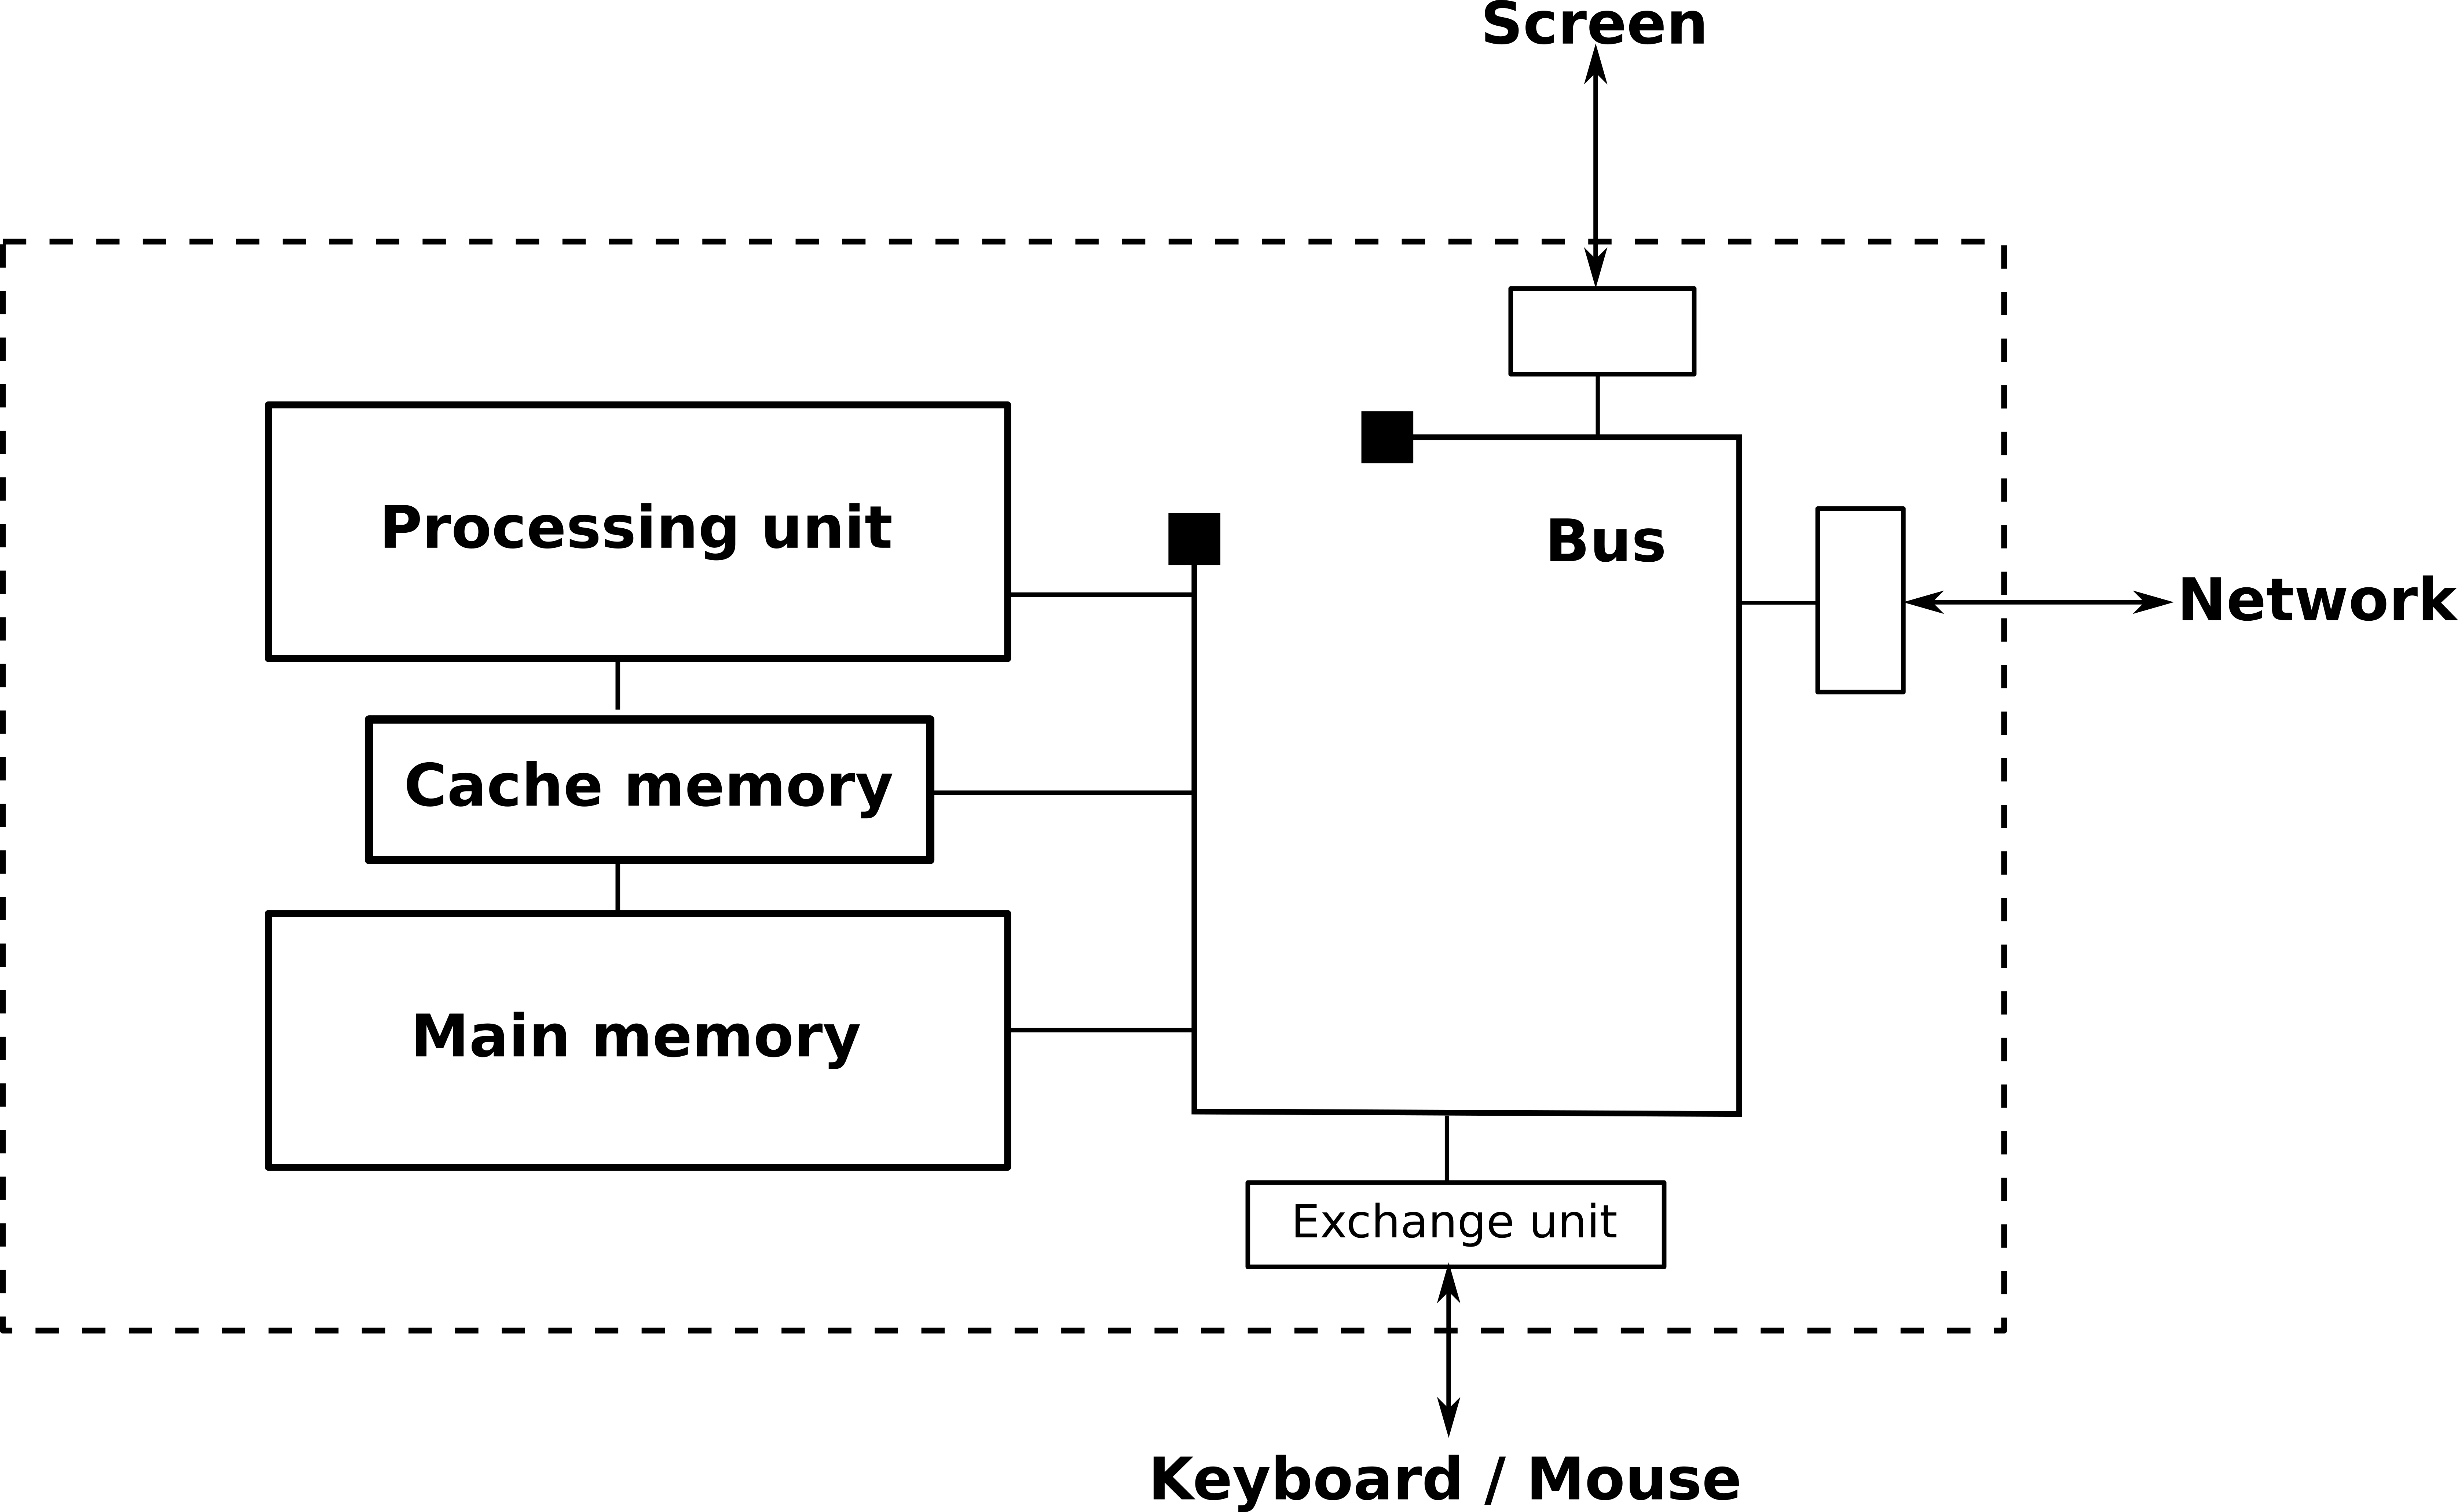
\includegraphics[scale=0.06]{images/von_neumann.png} 
     	%\vspace*{-0.5em}
		%\caption{Floating gate transistor cell}
	\end{figure}
	
	\end{center}	
		
	There are \textit{four} main components:
	
	\begin{enumerate}
	\item{Main memory (RAM)}
	\item{Processor unit (CPU)}
	\item{Peripheral control units}
	\item{Communication bus}	
	\end{enumerate}		
		
	\end{frame}		

	\section{Main memory}
	
	\subsection{Recall on binary notation}	
	
	\begin{frame}

	\begin{block}{Why binary?}
	At low level, a computer machine works in \textbf{binary} basis:
	\begin{itemize}
	\item{Numbers, characters, images, videos, ...: \textbf{all binary at low level}}
	\item{Underlying electronic components \textbf{can only manage 0s and 1s}}
	\end{itemize}		
	\end{block}
		
	Decimal basis to binary basis:
	\vspace*{0.5em}
	
	$1 = 2^0 = 1\times 2^0$ (simply: 1) 
	
	$10 = 8 + 2 = 2^3 + 2 = 1\times 2^3 + 0\times 2^2 + 1\times 2^1 + 0\times 2^0$ (simply: 1 0 1 0) 	
	
	\vspace*{0.5em}
	
	Binary basis to decimal basis:
	\vspace*{0.5em}

	$1\  1\  1 = 1\times 2^2 + 1\times 2^1 + 1\times 2^0 = 4 + 2 + 1 = 7$
	
	\vspace*{0.5em}
	
	\begin{block}{Note}
	\begin{itemize}
	\item{Each 0 or 1 in a binary notation is called a \textbf{\textit{bit}}}
	\item{Most significant bit: first bit (left), Least significant bit: last bit (right)}
	\end{itemize}
	\end{block}

	\end{frame}
	
	\begin{frame}
		
	The more we have bits, the more combinations we can handle:
	\vspace*{1em}
	\begin{columns}[c]
	\column{.5\textwidth}
	\begin{itemize}
	\item{With 2 bits:
		\begin{itemize}
			\item{0 0}
			\item{0 1}
			\item{1 0}
			\item{1 1}
		\end{itemize}
	}
	\item{With 3 bits:
		\begin{itemize}
		\item{0 0 0}
		\item{0 0 1}
		\item{0 1 0}
		\item{0 1 1}
		\item{1 0 0}
		\item{1 0 1}
		\item{1 1 1}	
		\end{itemize}
	}	
	\end{itemize}
	
	\column{.5\textwidth}
	\begin{itemize}
	\item{With 4 bits:
	\begin{itemize}
	\item{0 0 0 0}
	\item{0 0 0 1}
	\item{0 0 1 0}
	\item{0 0 1 1}
	\item{0 1 0 0}
	\item{0 1 0 1}
	\item{0 1 1 1}
	\item{1 0 0 0}
	\item{1 0 0 1}
	\item{1 0 1 1}
	\item{1 1 0 0}
	\item{1 1 0 1}
	\item{1 1 1 1}	
	
	\end{itemize}		
	}
	\end{itemize}
	\end{columns}
	
	\begin{block}{Note}
	This is why \textbf{having more bits generally = more speed or memory}
	\end{block}			
	
	\end{frame}	
	
	\subsection{How work the main memory}	
	
	\begin{frame}
	The \textit{main memory} works as follows (memory made of memory words):
	\vspace*{0.5em}
	
	\begin{center}
	\begin{figure}
		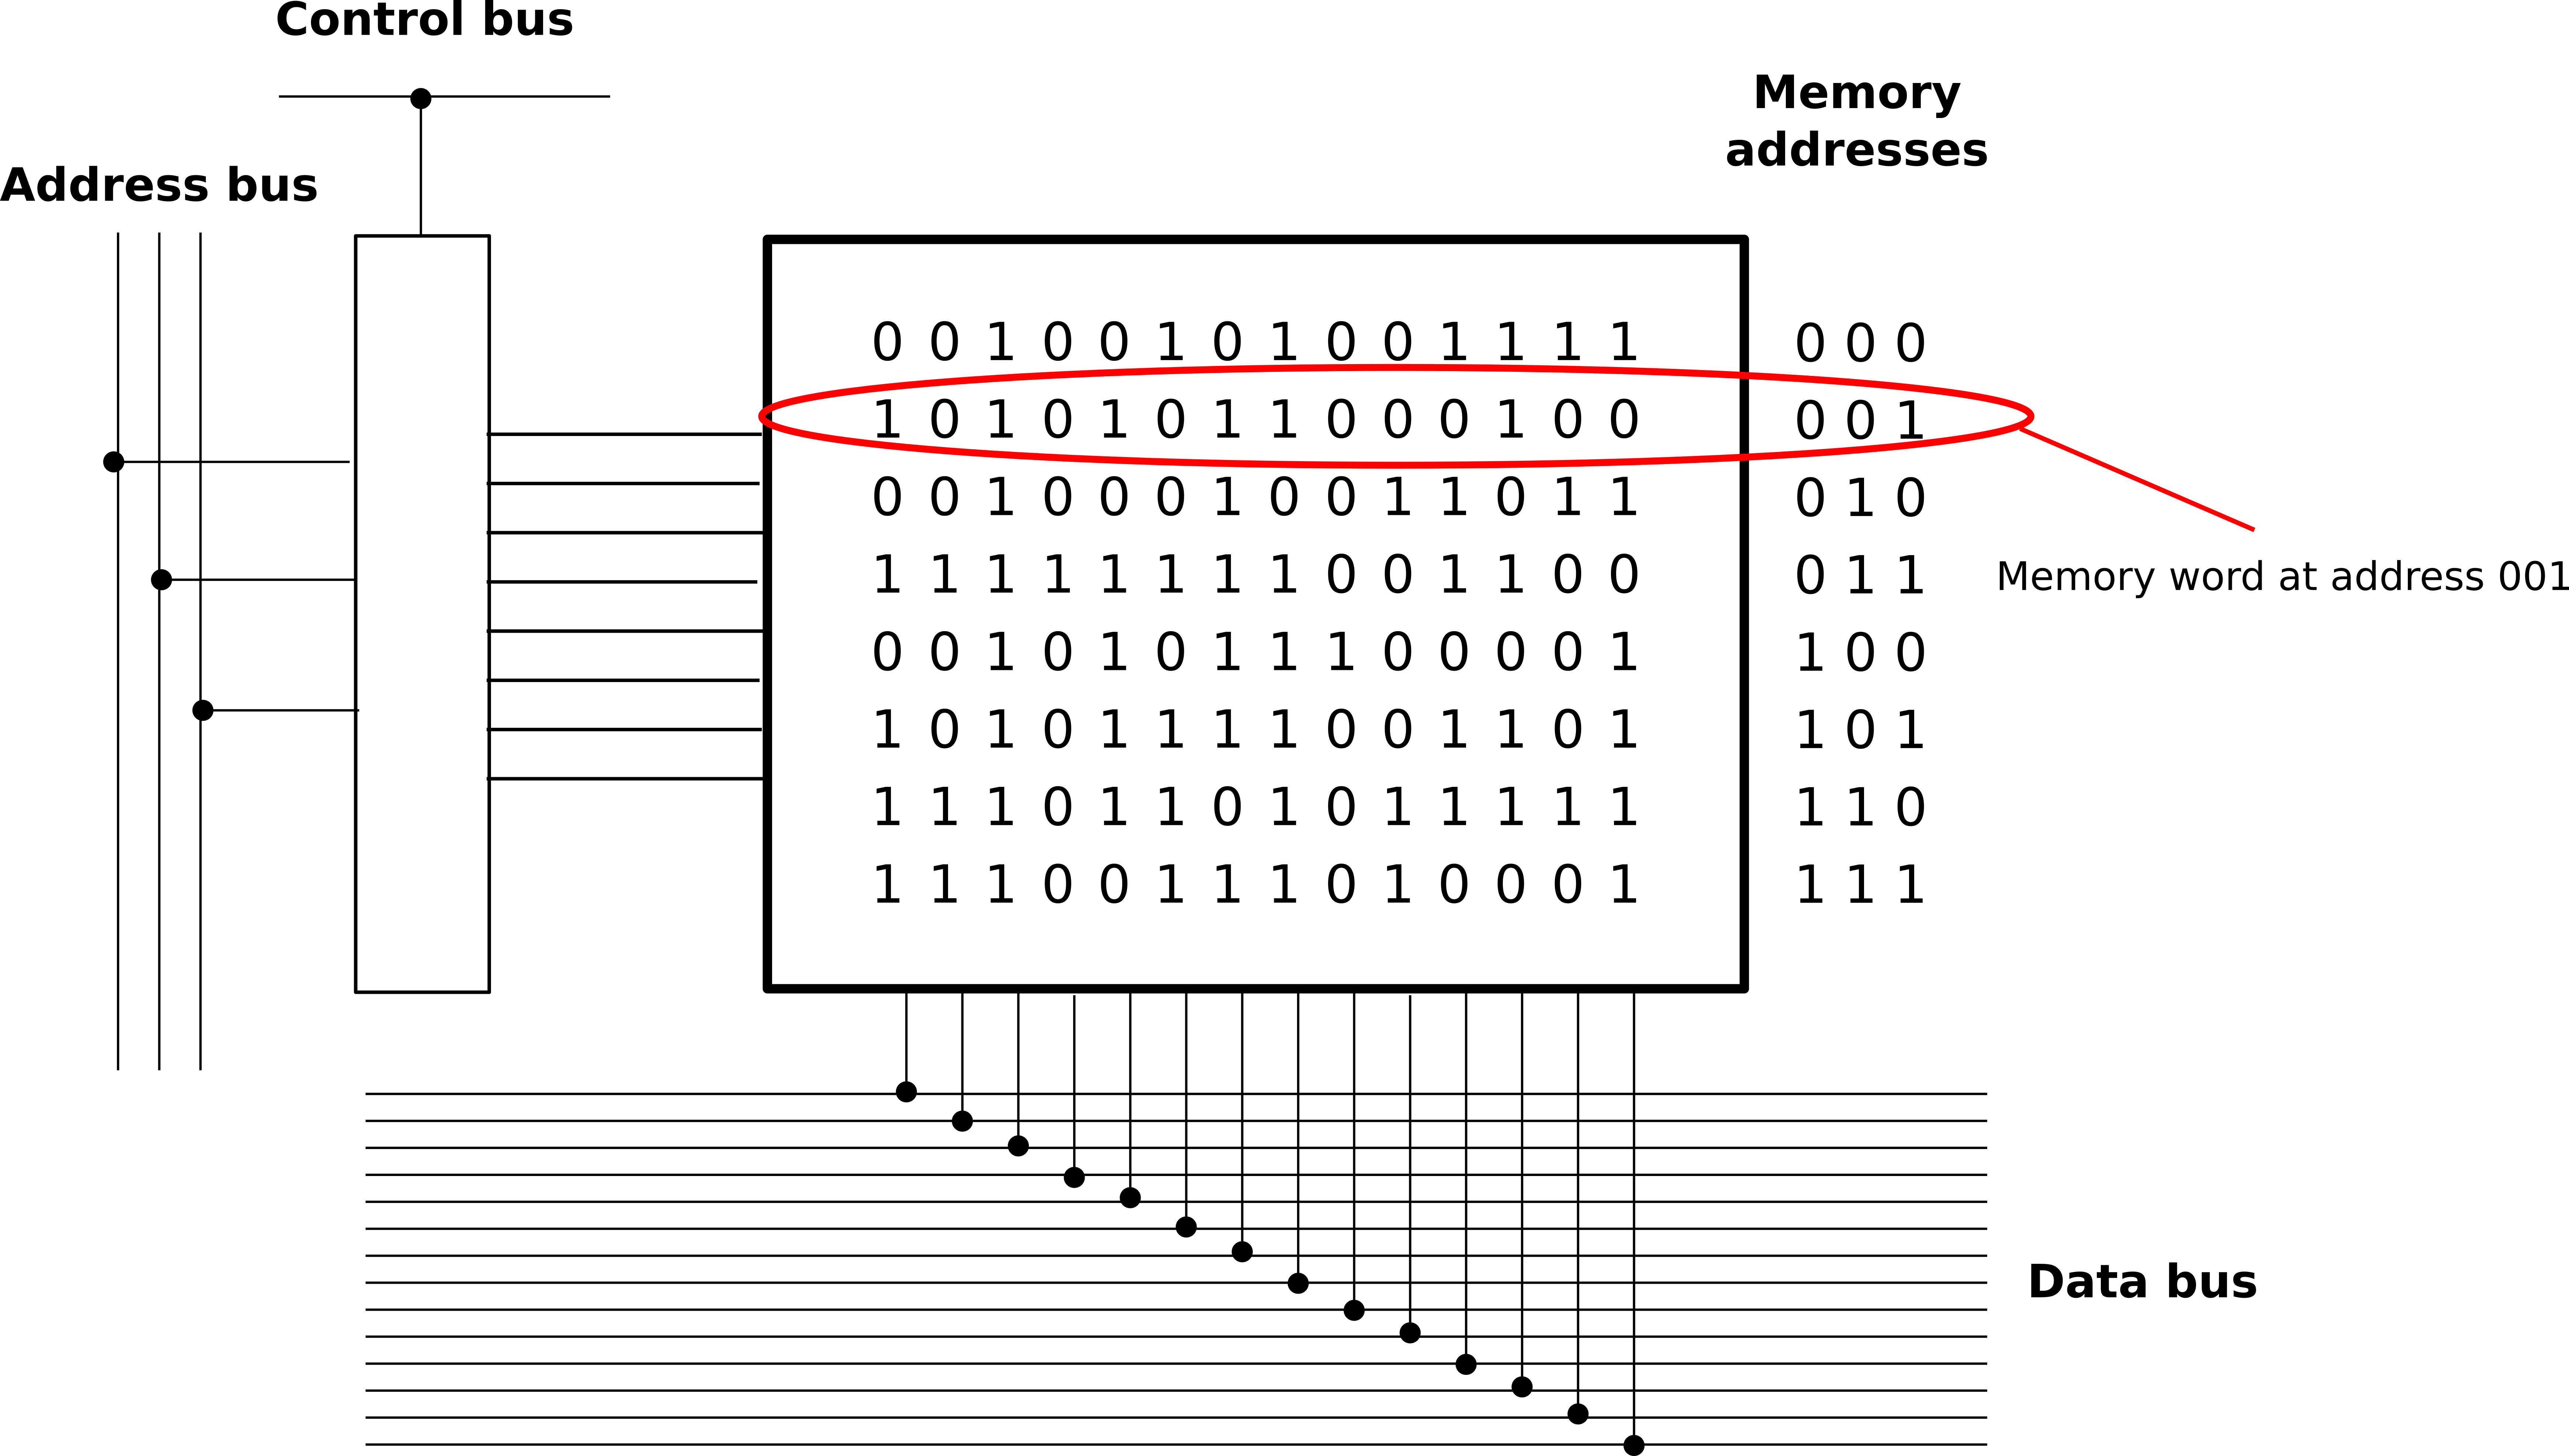
\includegraphics[scale=0.07]{images/main_memory.png} 
     	%\vspace*{-0.5em}
		%\caption{Floating gate transistor cell}
	\end{figure}
		
	\end{center}		
		
	\begin{itemize}
	\item{The \textit{address bus} allows memory word selection (given an address)}
	\item{The memory word is returned by the \textit{data bus} (here: word of 16 bits)}
	\item{The memory word is also written by the \textit{data bus}}
	\item{The \textit{control bus} handles read/write access (0 = read, 1 = write)}	
	\end{itemize}		
		
	\end{frame}
		
	\subsection{Instructions, data and memory words}
	
	\begin{frame}
	
	\textit{Instructions} are...:	
	\vspace*{.5em}
		\begin{itemize}
		\item{...stored \textbf{within memory words}}
		\item{...can occupy \textbf{one or more memory words}}
		\item{...\textbf{depend on the processor unit} (intel != ARM)}
		\item{...made of \textbf{opcodes} and one or more \textbf{addressing mode(s)}:
			\begin{itemize}
				\item{\textit{opcode}: binary code specifying an operation (add, mult, etc.)}
				\item{\textit{addressing mode}: binary address of other memory words with data}
			\end{itemize}					
		}
		
		\end{itemize}			
	
	\vspace*{0.5em}
	
	Examples:

	\begin{center}
	\begin{figure}
		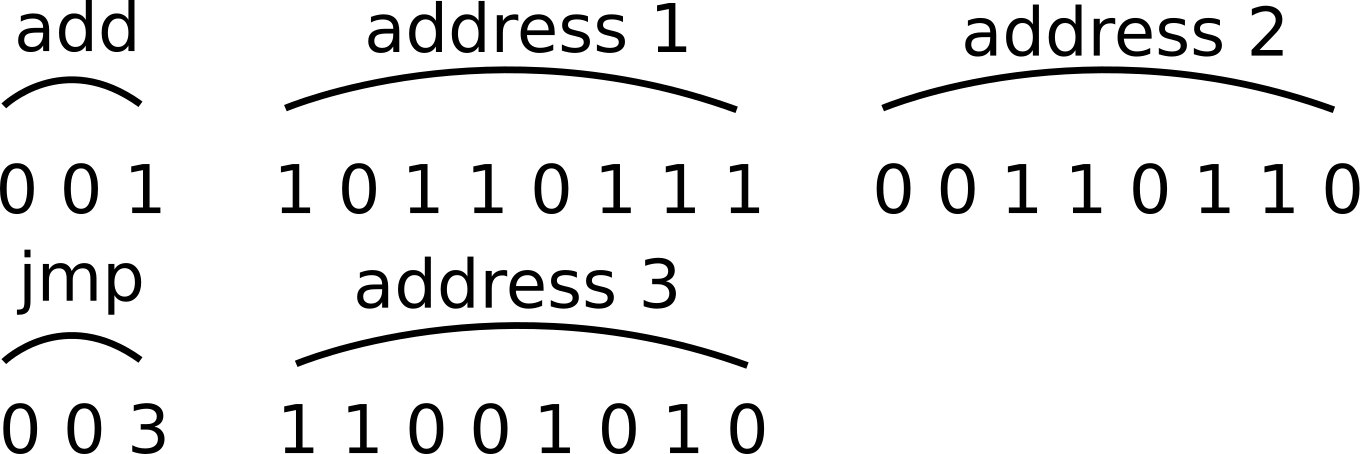
\includegraphics[scale=0.2]{images/instruction_example_1.png} 
     	%\vspace*{-0.5em}
		%\caption{Floating gate transistor cell}
	\end{figure}
		
	\end{center}		
		
	Data are...
	\begin{itemize}
	\item{...also stored \textbf{within memory words}}
	\item{...can also occup \textbf{one or more memory words}}
	\end{itemize}		

	\end{frame}

	\subsection{Communication bus}
	
	\begin{frame}
	
	\begin{block}{What is a bus?}
	Buses allow \textbf{information exchanges} and \textbf{data transfer}
	\end{block}	

	\vspace*{1em}	
	
	There are three different buses:
	
	\vspace*{1em}
	
	\begin{enumerate}
	\item{\textit{address bus}: transport memory word addresses}
	\item{\textit{control bus}: transport control operations (read/write for example)}	
	\item{\textit{data bus}: transport data to read or write from memory}
	\end{enumerate}		
	
	\begin{block}{Note about the address bus}
	\begin{itemize}
	\item{The more bits, the more memory word addresses can be covered}
	\item{But memory size correlated to number of bits in memory words!}
	\end{itemize}
	\end{block}	
	
	\end{frame}

	\section{Processor unit}
	\subsection{General presentation}	
	
	\begin{frame}
	
	\begin{block}{What is the goal of the processor unit?}
	The processor unit \textbf{executes instructions} stored in the \textit{main memory}	
	\end{block}
	
	A processor unit (or CPU) is composed of three sub-components:
	\vspace*{-1.5em}
	
	\begin{columns}[c]
	
	\column{.5\textwidth}	
	
	\begin{enumerate}
		\item{Arithmetic Logic Unit (ALU)}
		\item{Registers}
		\item{Control Units (CU)}
	\end{enumerate}		

	\column{.5\textwidth}
	
	\begin{center}
	\begin{figure}
		\includegraphics[scale=0.032]{images/cpu.png} 
     	%\vspace*{-0.5em}
		%\caption{Floating gate transistor cell}
	\end{figure}
		
	\end{center}	

	
	\end{columns}	
		
		
	\end{frame}

	\subsection{Arithmetic Logic Unit (ALU)}
	
	\begin{frame}
	
	\begin{exampleblock}{Goal}
	Perform arithmetic operations on two values
	\end{exampleblock}	
	
	\vspace*{-1.5em}	
	
	\begin{columns}[c]
	
	\column{.5\textwidth}
	
	\begin{center}
	\begin{figure}
		\includegraphics[scale=0.032]{images/cpu_alu.png} 
     	%\vspace*{-0.5em}
		%\caption{Floating gate transistor cell}
	\end{figure}
		
	\end{center}	

	\column{.5\textwidth}

	\begin{itemize}
	\item{1st value placed in register \textit{Y1}\footnotemark[1]}
	\item{2nd value placed in register \textit{Y2}\footnotemark[1]}
	\item{operation performed on the pair}
	\item{result placed in register \textit{Z}\footnotemark[1]}
	\item{\textit{PSW}\footnotemark[1]: signal capacity overflows}	
	\end{itemize}

	\end{columns}	
		
	\footnotetext[1]{\textit{Y1}, \textit{Y2}, \textit{PSW} and \textit{Z} are \textit{special} registers: they have a specific use}		
		
	\end{frame}	
	
	\subsection{Registers Unit}	
	
	\begin{frame}	
	
	\begin{exampleblock}{Goal}
	The registers unit store general information (with high speed access)
	\end{exampleblock}	
		
	\vspace*{-1.5em}		
		
	\begin{columns}[c]
	
	\column{.5\textwidth}
	
	\begin{center}
	\begin{figure}
		\includegraphics[scale=0.032]{images/cpu_registers.png} 
     	%\vspace*{-0.5em}
		%\caption{Floating gate transistor cell}
	\end{figure}
		
	\end{center}	

	\column{.5\textwidth}

	Registers are...
	\vspace*{0.5em}
	\begin{itemize}
	\item{...filled by the internal data bus}
	\item{...read from the internal data bus}	
	\end{itemize}

	\end{columns}	
	
	\end{frame}
	
	\subsection{Control Unit (CU)}
	
	\begin{frame}

	\begin{exampleblock}{Goal}
	Execute instructions using the \textit{ALU} and the \textit{registers unit}	
	\end{exampleblock}

	\vspace*{-1.5em}

	\begin{columns}[c]
	
	\column{.5\textwidth}
	
	\begin{center}
	\begin{figure}
		\includegraphics[scale=0.032]{images/cpu_cu.png} 
     	%\vspace*{-0.5em}
		%\caption{Floating gate transistor cell}
	\end{figure}
		
	\end{center}	

	\column{.5\textwidth}

	\begin{itemize}
	\item{\textit{RDO}\footnotemark[2]: register storing data}
	\item{\textit{RAD}\footnotemark[2]: register storing addresses}
	\item{\textit{RI}\footnotemark[2]: register storing instruction}
	\item{\textit{CO}\footnotemark[2]: register with next address}
	\item{\textit{decoder}: decode content of \textit{RI}}
	\item{\textit{sequencer}: commands $\Rightarrow$ ALU}		
	\end{itemize}

	\end{columns}	
	
	\footnotetext[2]{\textit{RDO}, \textit{RAD}, \textit{RI} and \textit{CO} are specific registers}	
	
	\end{frame}	
	
	\begin{frame}
	
	With more details, when the CPU has to execute an instruction:	
	
	\vspace*{0.5em}
	
	\begin{enumerate}
	\item{Content of \textbf{CO is placed in RAD}}
	\item{\textbf{Read is triggered} thanks to the control bus}
	\item{\textbf{RDO receives instruction} (data bus)}
	\item{Content of \textbf{RDO placed in RI}}
	\item{Instruction \textbf{decoded in decoder}}
	\item{Set of \textbf{commands sent (timer rythm) to ALU} (sequencer)}
	
	\end{enumerate}
	
	\vspace*{0.5em}	
	
	When the CPU has to read a data:
	
	\vspace*{0.5em}	
		
	\begin{enumerate}
	\item{Address \textbf{placed in RDA}}
	\item{\textbf{Read is triggered} thanks to control bus}
	\item{\textbf{RDO receives data}}
	\item{\textbf{Data placed in general registers or ALU registers}}
	\end{enumerate}			
		
	
	\end{frame}	
	
	\section{Exchange units}
	\subsection{General presentation}	
	
	\begin{frame}
	
	\textit{Exchange units}...
	
	\begin{itemize}
	
	\item{...are in \textbf{communication with the processor unit} (internal bus)}
	\item{...are also in \textbf{communication with the peripherals}}	
	
	\end{itemize}		
	
	\begin{center}
	\begin{figure}
		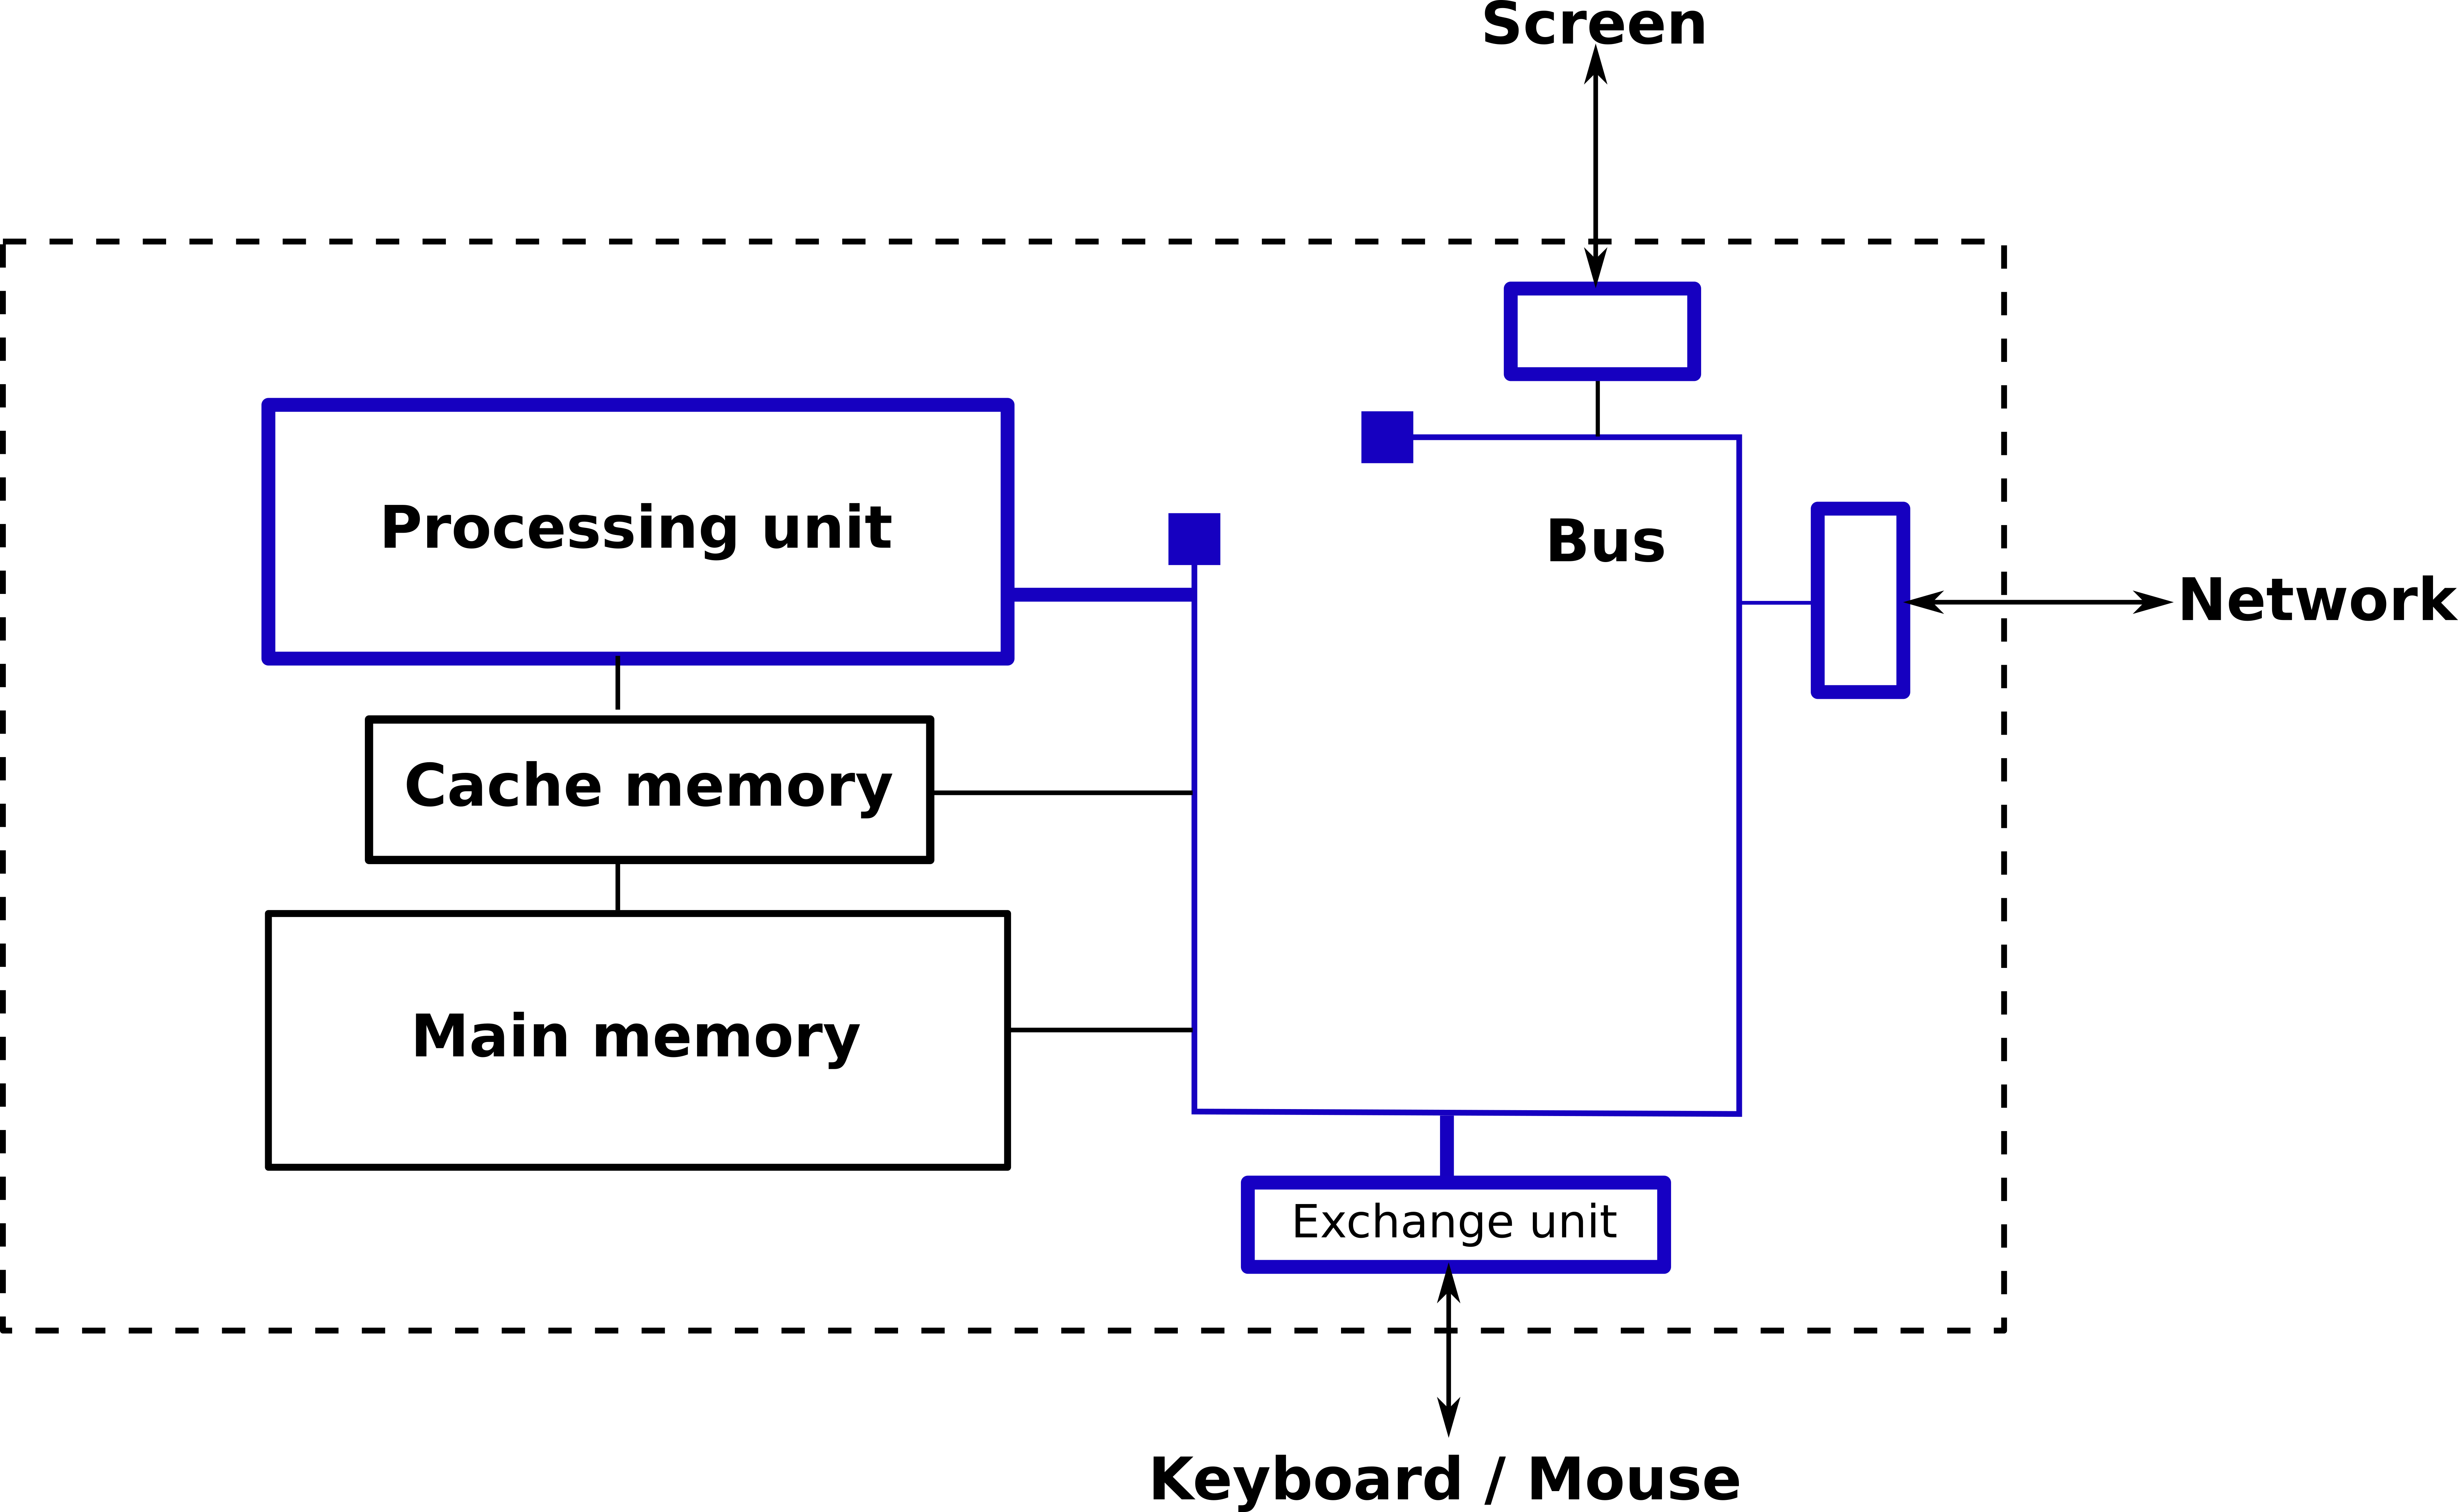
\includegraphics[scale=0.07]{images/von_neumann_2.png} 
     	%\vspace*{-0.5em}
		%\caption{Floating gate transistor cell}
	\end{figure}
		
	\end{center}	
	
	
	\begin{exampleblock}{Goal}	
	\begin{itemize}
	\item{Ensure standard comm. between \textit{processor unit} and \textit{peripherals}}
	\item{Exchange unit: takes care of variety of hardware}
	\end{itemize}
	
	\end{exampleblock}
		
	\end{frame}		

	\section{Program production chain}
	\subsection{General presentation}	
	
	\begin{frame}	
	
	The \textit{program production chain} is at follows:
	\vspace*{1em}
	\begin{enumerate}
	\item{High-level code is written using an \textbf{editor}}
	\item{Code is \textbf{complied} into binary objects}
	\item{Objects are \textbf{linked} together and with libraries}
	\item{Program is \textbf{loaded in main memory}}	
	\end{enumerate}		
	
	\begin{center}
	\begin{figure}
		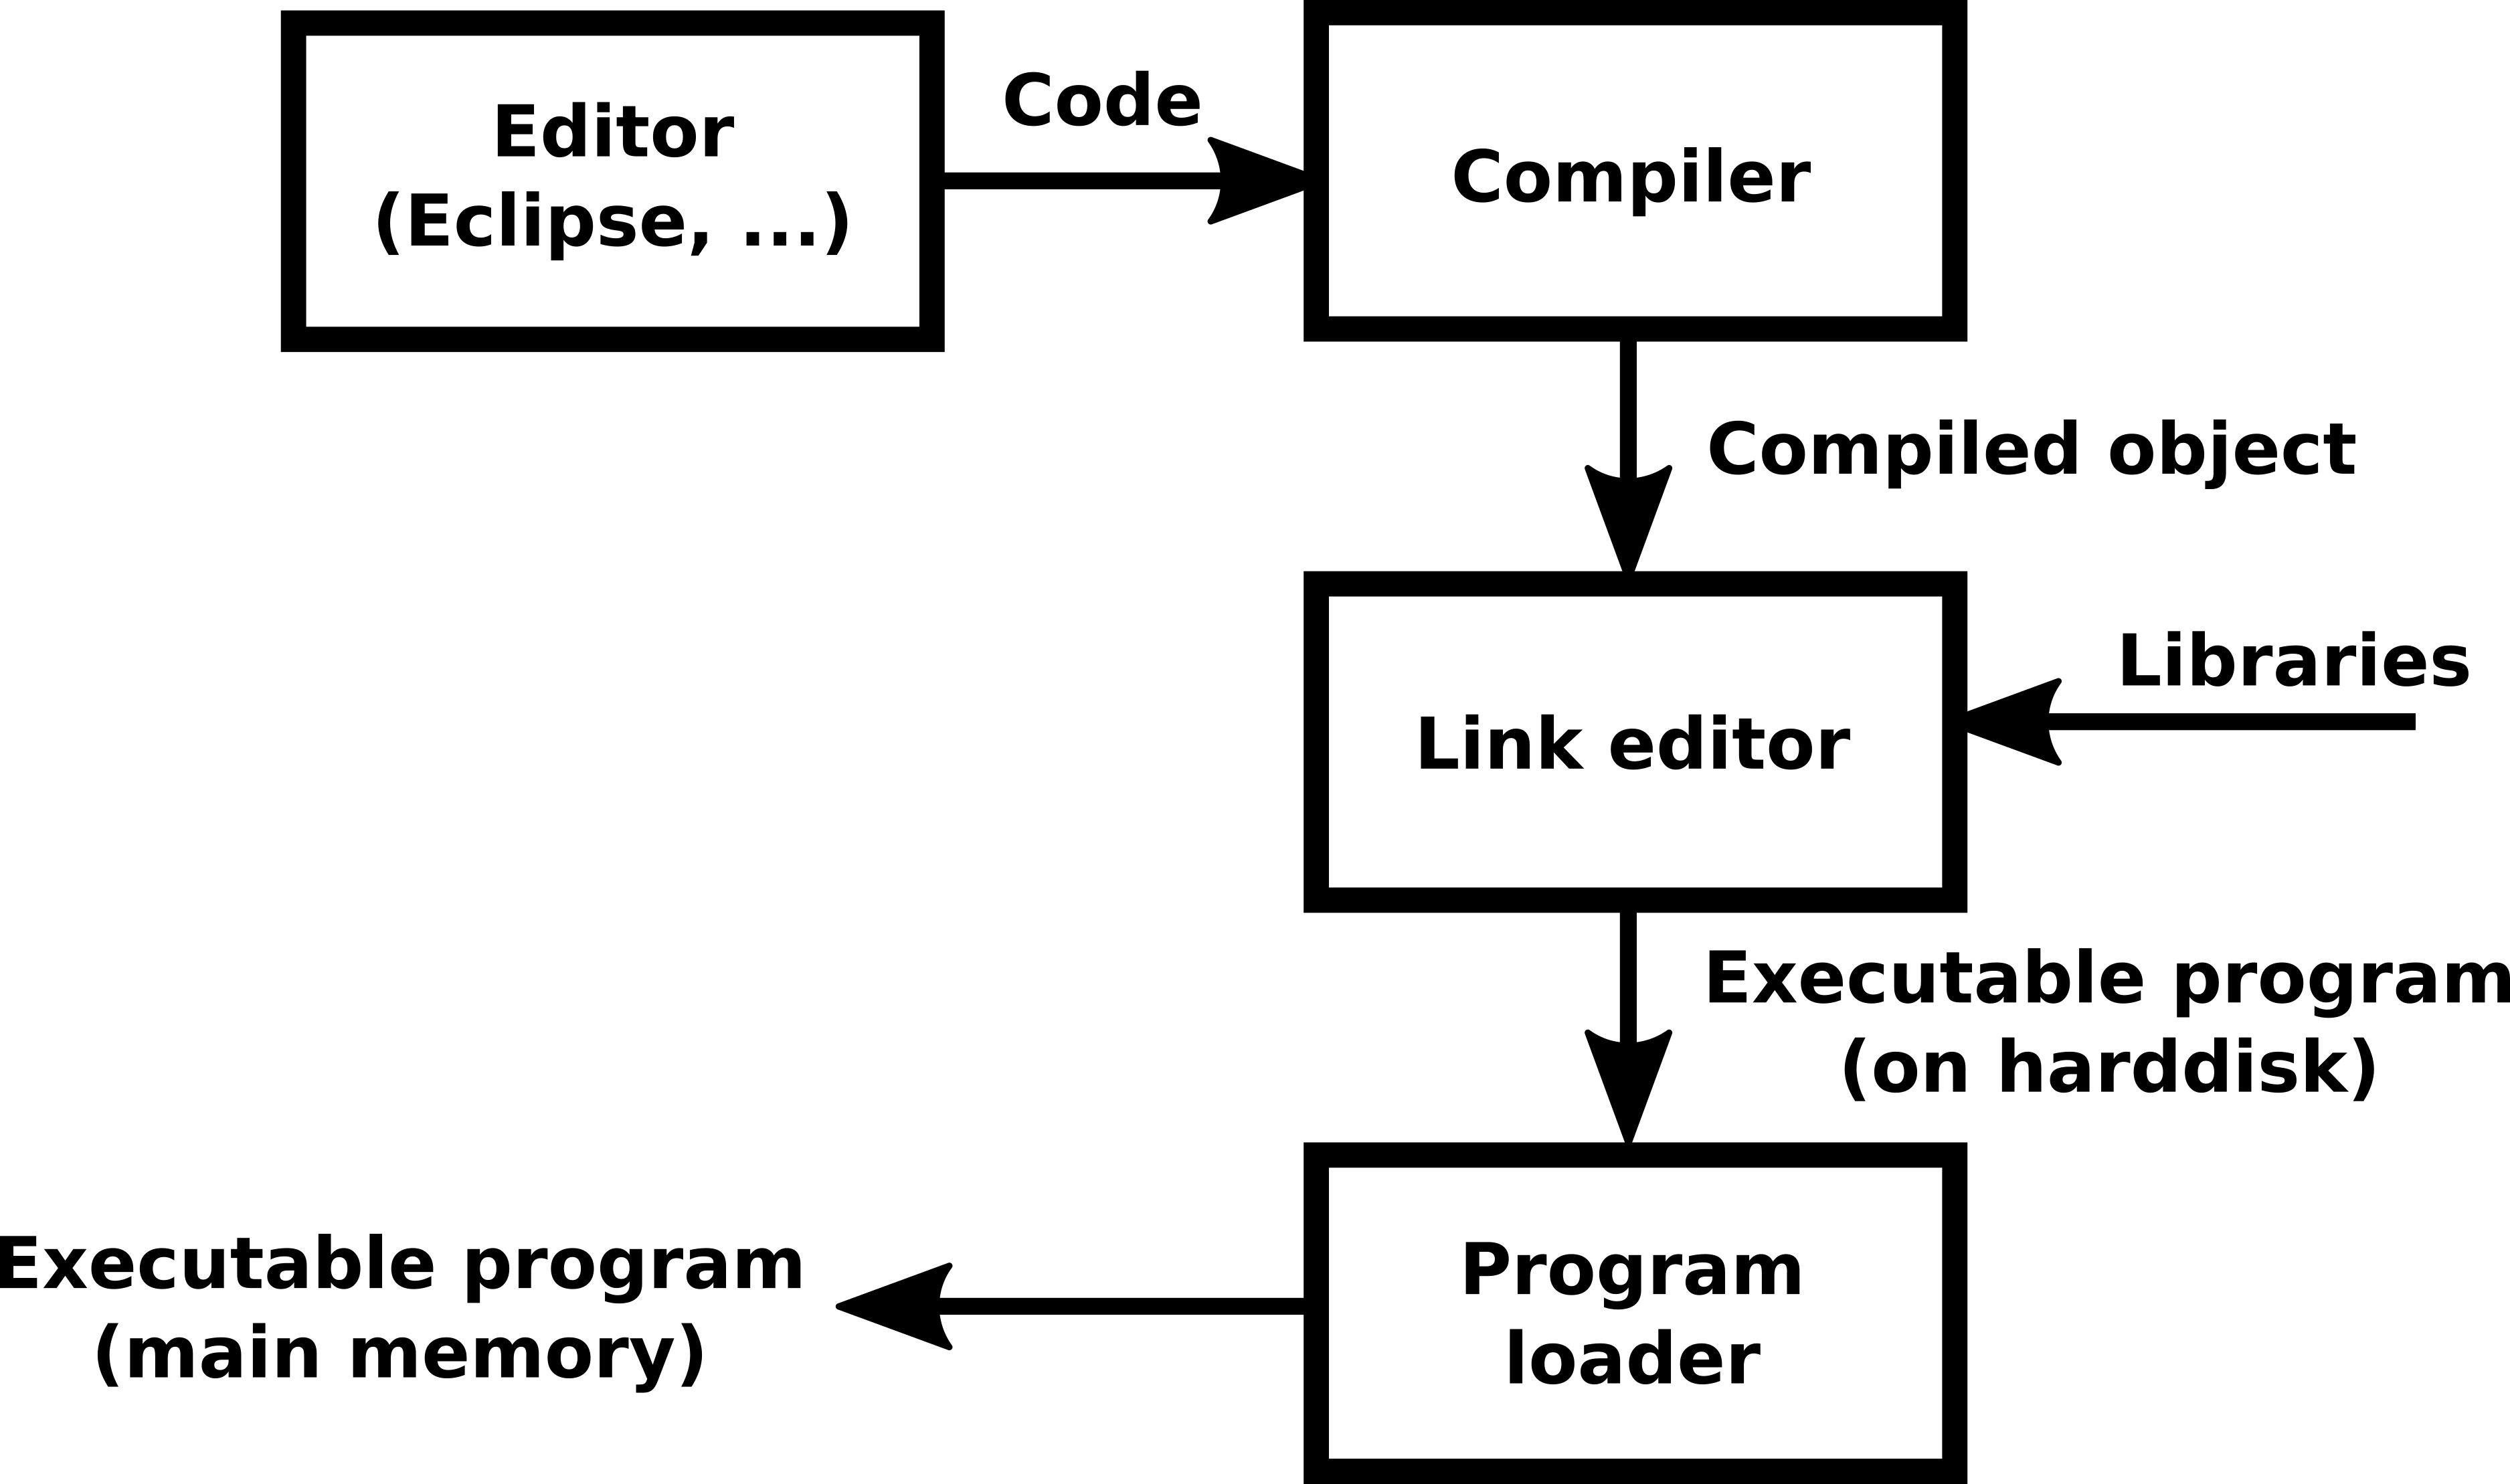
\includegraphics[scale=0.09]{images/chain.png} 
     	%\vspace*{-0.5em}
		%\caption{Floating gate transistor cell}
	\end{figure}
		
	\end{center}
	
	\end{frame}
	
	\subsection{Compilation}
	
	\begin{frame}
	\begin{block}{What is compilation?}
	It consists in transforming \textbf{human-readable source code into binary code}
	\end{block}
	\vspace*{1em}
	
	\begin{center}
	\begin{figure}
		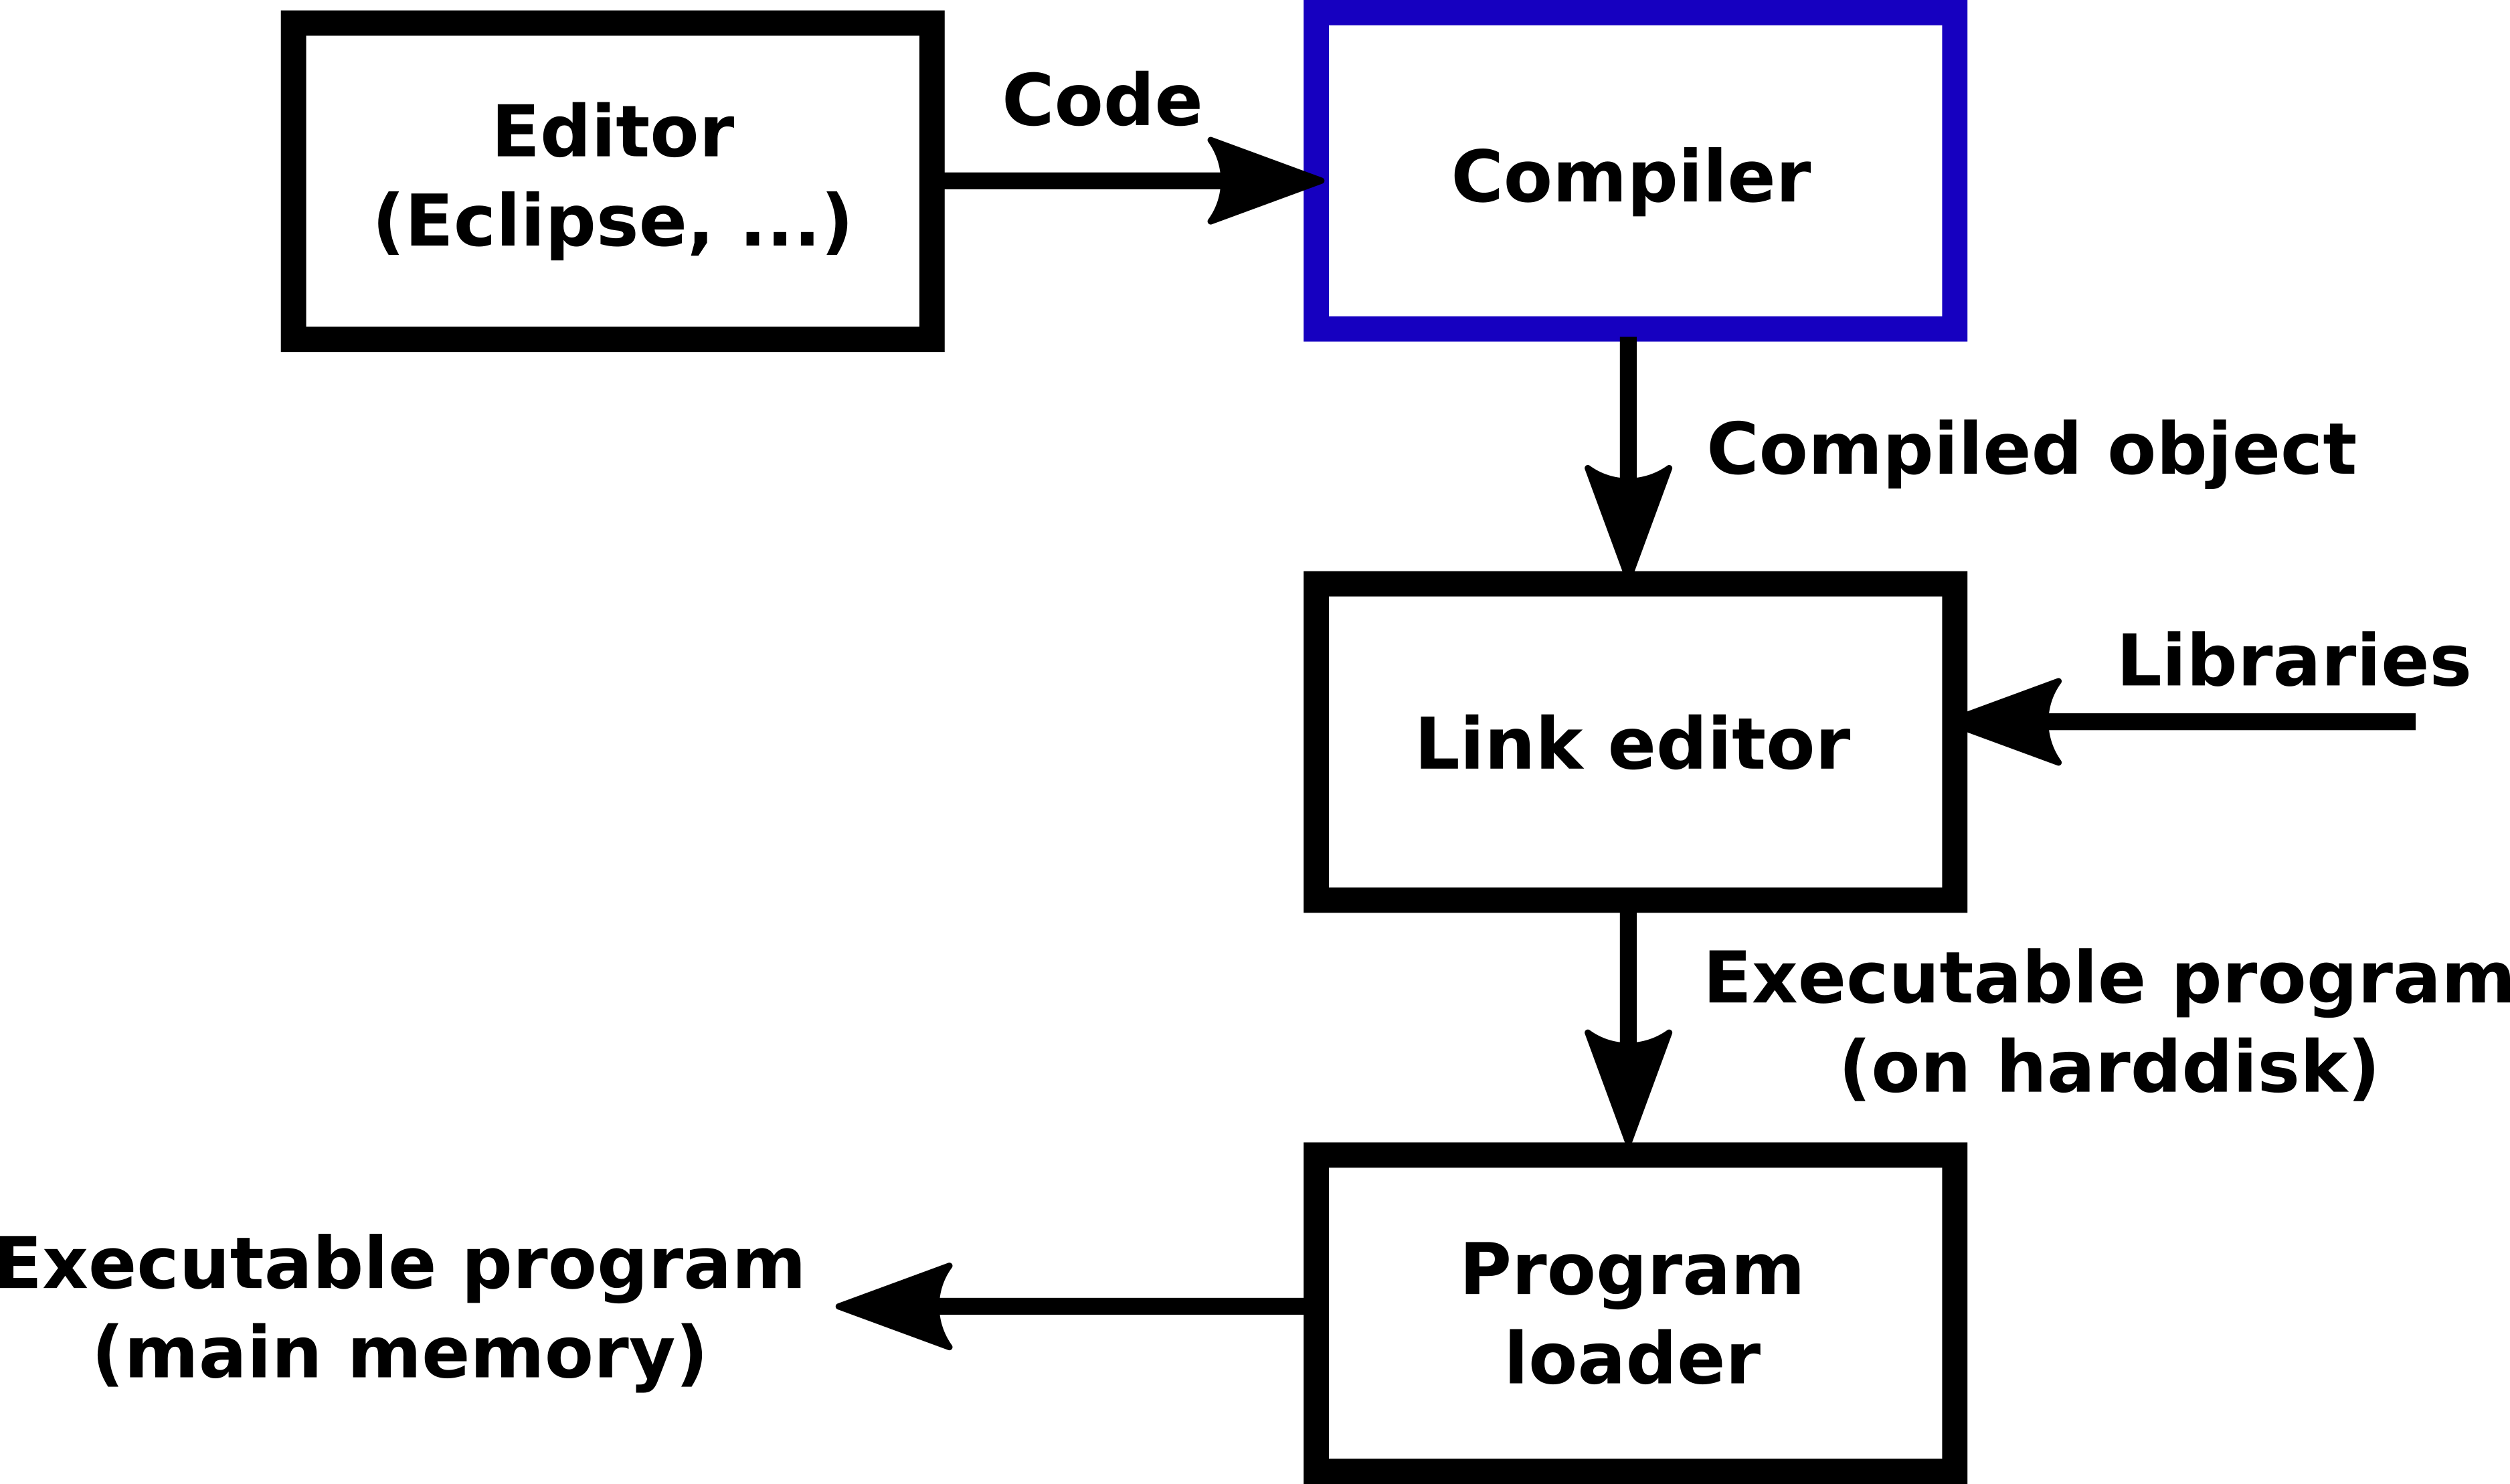
\includegraphics[scale=0.09]{images/chain_c.png} 
     	%\vspace*{-0.5em}
		%\caption{Floating gate transistor cell}
	\end{figure}
		
	\end{center}
	
	Compiling consists in four steps:
	\vspace*{1em}	
	
	\begin{enumerate}
	\item{the \textbf{lexical analysis}}
	\item{the \textbf{syntactic analysis}}
	\item{the \textbf{semantic analysis}}
	\item{the \textbf{code optimization} and \textbf{code generation}}
	\end{enumerate}		

	\end{frame}	
	
	\begin{frame}
	
	\begin{block}{What is the lexical analysis?}
	lexical analysis = \textbf{recognizing the words of the language}
	\end{block}
	\vspace*{1em}
	A high-level programming language is made of:
	\vspace*{1em}
	\begin{itemize}
	\item{an \textbf{alphabet} (set of authorized symbols)
		\begin{itemize}
			\item{characters, numbers, punctuation, etc.}
			\item{examples: !?=/\{\};:-()abcdef..z1234..9}
		\end{itemize}			
	}
	\item{\textbf{words} (made of elements of the alphabet):
		\begin{itemize}
		\item{examples: int,char,const,etc.}
		\end{itemize}			
	}	
	\item{\textbf{phrases}:
		\begin{itemize}
			\item{\textbf{groups} of language words}
			\item{respecting a set of \textbf{grammatical rules}}
		\end{itemize}			
	}
	
	\end{itemize}
	
	\end{frame}

	\begin{frame}

	Examples of \textit{grammatical rules} (following the rules of Backus-Naur):
	\vspace*{1em}
	
	<PROGRAM> => PROGRAM <IDENTIFIER> <PROGRAM BODY> 
	
	<PROGRAM BODY> => <OTHER DECLARATIONS> BEGIN <NEXT DECLARATIONS> END
	
	<NEXT DECLARATIONS> => <DECLARATION> or <DECLARATION> <NEXT DECLARATIONS>

	<DECLARATION> => INT <IDENTIFIER>;
	
	<TERM> => <INTEGER> or <IDENTIFIER>

	<OPERATOR> => + or – or * or /

	<IDENTIFIER> => <CHARACTER> or <CHARACTER> <NUMBER>

	<INTEGER> => <NUMBER> or <NUMBER> <CHARACTER>

	<OPERATION> => <IDENTIFIER> = <TERM> <OPERATOR> <TERM>; or <IDENTIFIER> = <TERM>;

	<NEXT OPERATION> => <OPERATION> or <OPERATION> <NEXT OPERATION>

	<CHARACTER> =>  A or B or C or D, ..., Z

	<NUMBER> => 0 or 1 or 2 or 3, ...9 	
	
	\end{frame}

	\begin{frame}

	\begin{block}{What does the syntactic analysis?}
	\textbf{Analyze symbols} returned by the lexical analysis and \textbf{check the syntax}
	\end{block}
	
	\vspace*{1em}
	
	Example 1 (program with correct syntax):
	
	\vspace*{1em}
	
	\begin{columns}[c]
	
	\column{.4\textwidth}
	PROGRAM myProgram
	
	INT VAR1;
		
	INT RESULT;	
	
	BEGIN	
	
	VAR1 = 20;
	
	RESULT = VAR1 * 2;
	
	END
	\column{.6\textwidth}	
	
	\begin{center}
	\begin{figure}
		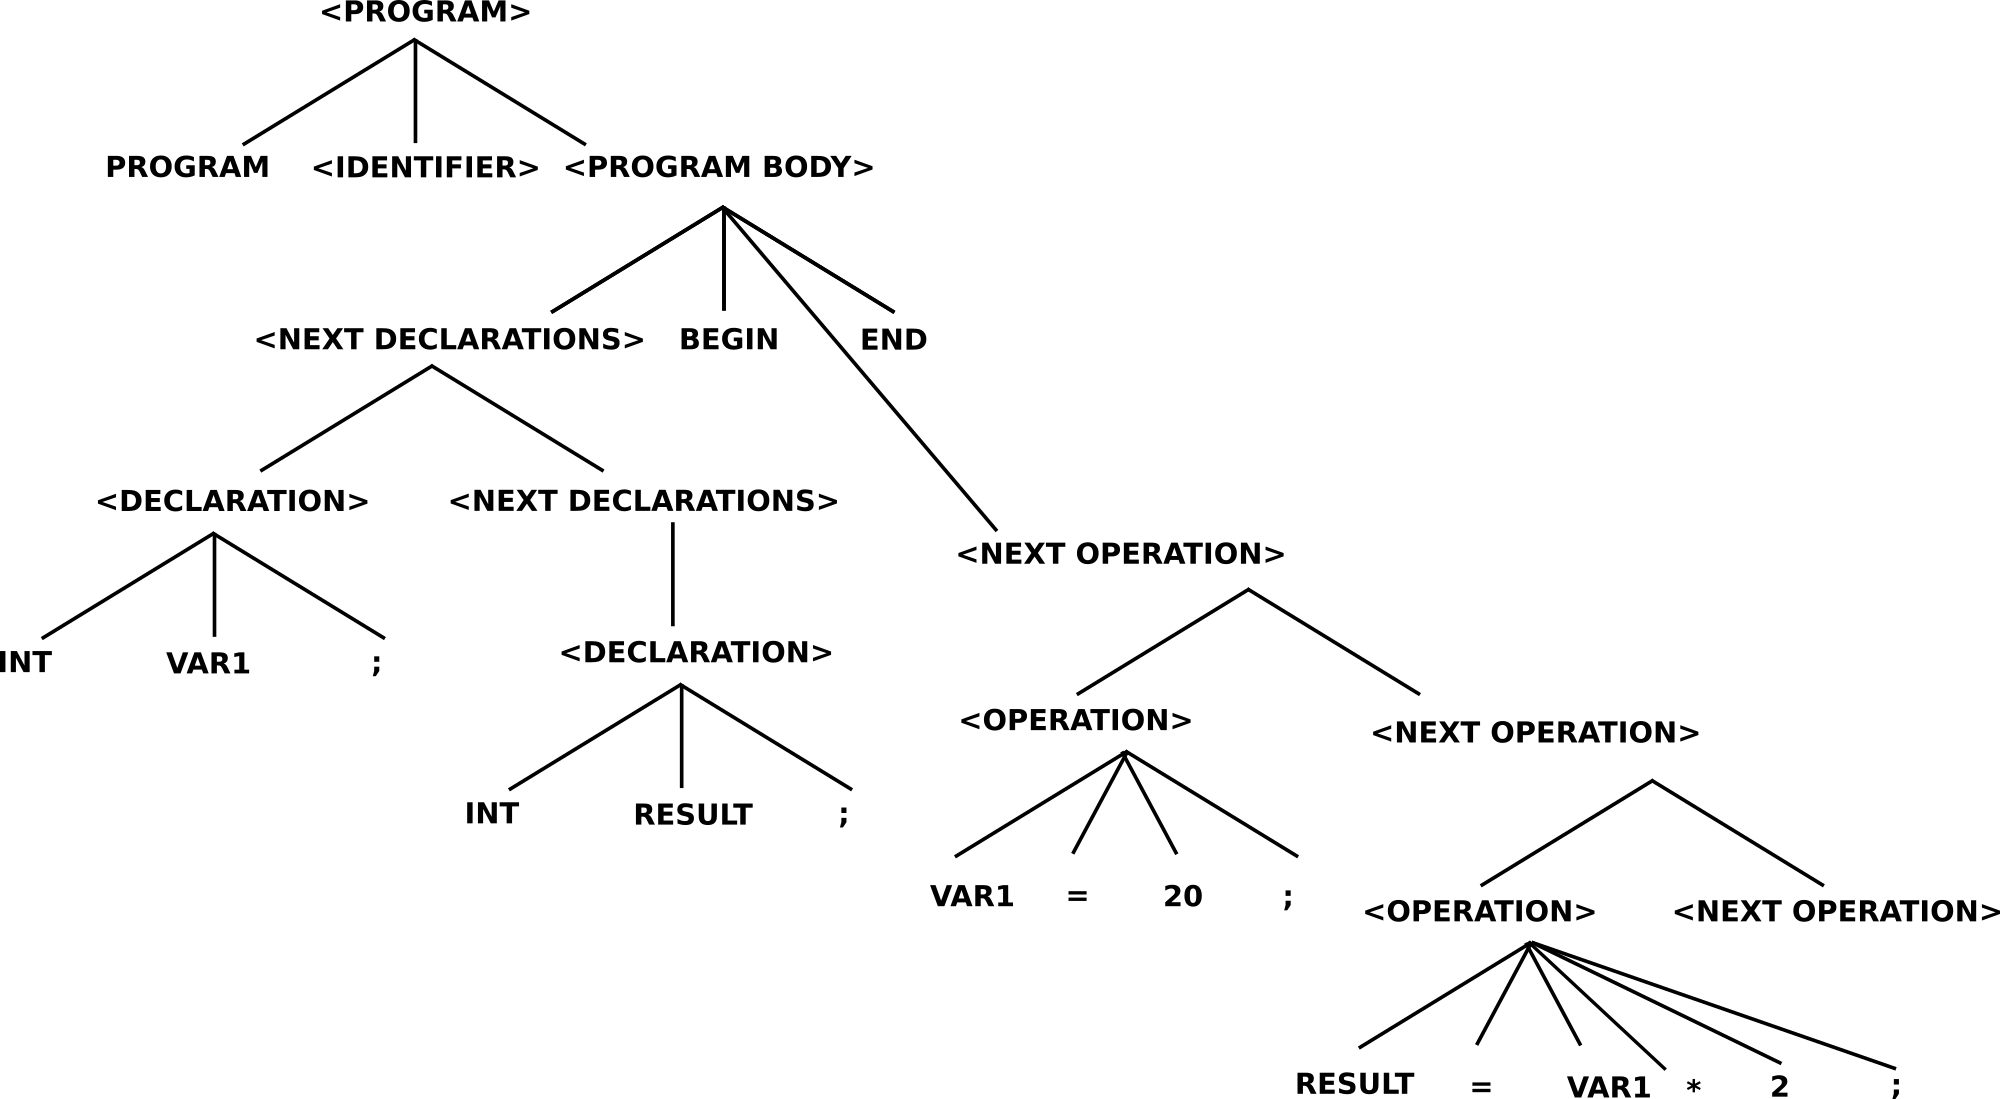
\includegraphics[scale=0.03]{images/graph_code.png} 
     	%\vspace*{-0.5em}
		%\caption{Floating gate transistor cell}
	\end{figure}
		
	\end{center}
	
	\end{columns}
		
	\end{frame}

	\begin{frame}
	Example 2 (program with a syntax error):
	
	\vspace*{1em}
	
	\begin{columns}[c]
	
	\column{.4\textwidth}
	PROGRAM myProgram
	
	INT VAR1;
		
	INT RESULT;	
	
	BEGIN	
	
	VAR1 = 20;
	
	RESULT = VAR1 * 2
	
	END
	\column{.6\textwidth}	
	
	\begin{center}
	\begin{figure}
		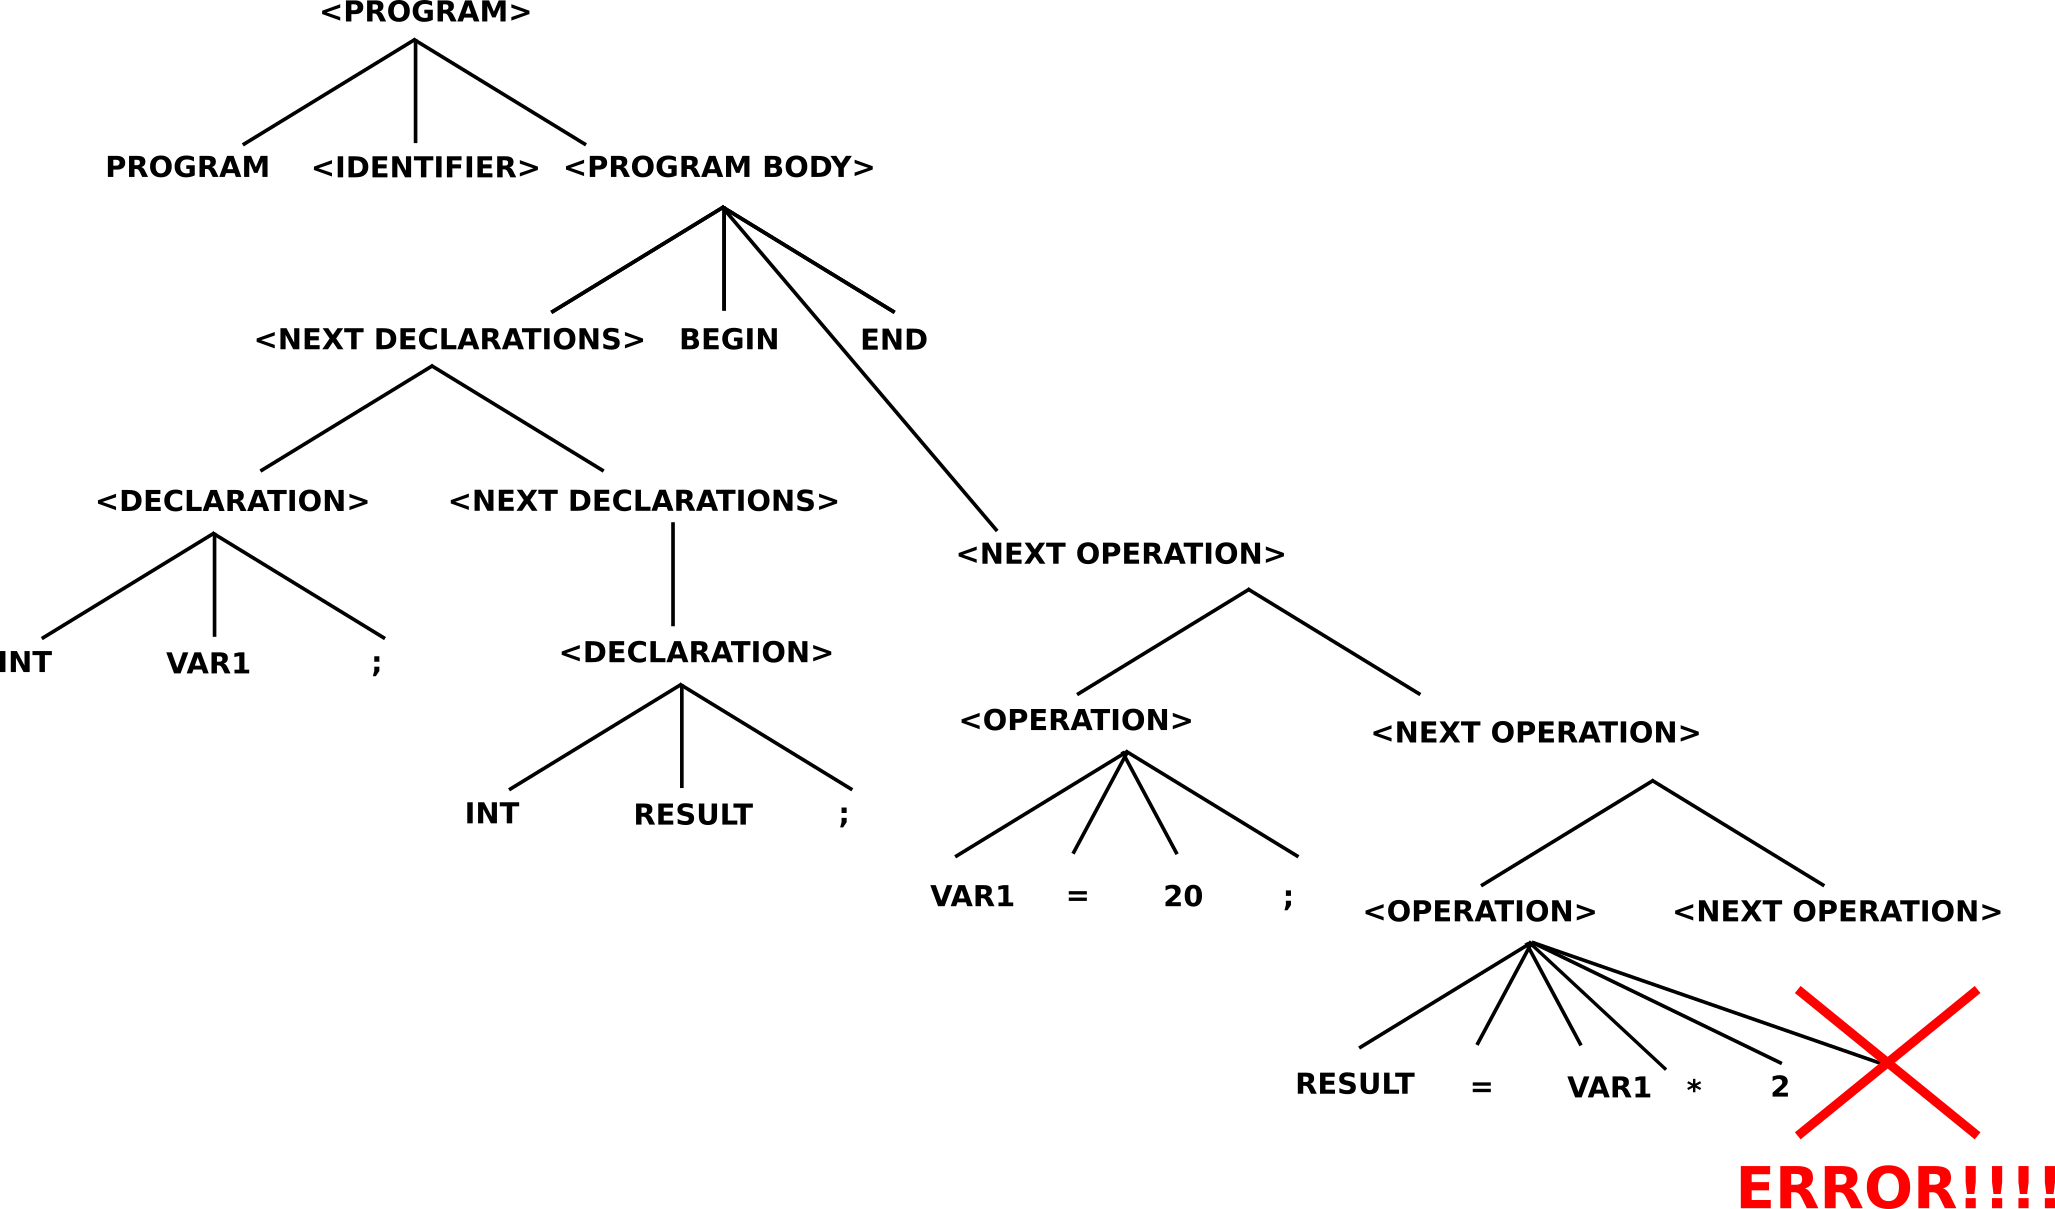
\includegraphics[scale=0.03]{images/graph_code_error.png} 
     	%\vspace*{-0.5em}
		%\caption{Floating gate transistor cell}
	\end{figure}
		
	\end{center}
	
	\end{columns}		
	
	\end{frame}

	\begin{frame}
	
	\begin{block}{What does the semantic analysis?}
	It associates a purpose to the phrases by:
	\begin{itemize}
	\item{recognizing the objects and their \textbf{properties} (type, time of life, etc.)}
	\item{checking that \textbf{objects are properly used}}
	\end{itemize}		
	\end{block}	
	\vspace*{1em}
	Examples of common object misusages detected by semantic analysis:
	\vspace*{1em}
	\begin{itemize}
	\item{objects declared several times}
	\item{objects used whereas deleted before}
	\item{object declared with wrong type}
	\item{etc...}
	\end{itemize}		
	
	\end{frame}

	\begin{frame}
	
	\begin{block}{What is the \textit{code generation} and \textit{optimization}?}	
	The final step of the \textit{compilation} generating a \textit{binary relocatable file}\footnotemark[3]
	\end{block}

	It starts by getting a \textbf{table of symbols} of the program, example:
	\begin{center}
	\begin{tabular}{|c|c|c|c|}
	\hline
	Object name & Type & Size & Address \\ \hline
	VAR1 & INT & 4 bytes & (0) \\ \hline
	RESULT & INT & 4 bytes & (4) \\ \hline
	\end{tabular}	
	\end{center}	
	
	Then, by transforming the code into an \textbf{intermediary code}:
	\vspace*{1em}	
	
	\begin{columns}[c]
	\column{.5\textwidth}
	\begin{tiny}
	
	Original code:
	\vspace*{0.5em}	
	
	PROGRAM myProgram
	
	INT VAR1;
		
	INT RESULT;	
	
	BEGIN	
	
	VAR1 = 20;
	
	RESULT = VAR1 * 2
	
	END	
	
	\end{tiny}
	\column{.5\textwidth}
	\begin{tiny}
	Intermediary code:
	\vspace*{.5em}
	
	(0)
	
	(4)
	
	INIT (0) 20
	
	MULT (4) (0) 2
	
	STOP 
	
	\end{tiny}
	\end{columns}
	\footnotetext[3]{relocatable means: the addresses of the objects start at 0}	
			
	\end{frame}
	
	\begin{frame}
	
	The \textit{intermediary code} is then optimized:
	\vspace*{1em}

	\begin{columns}[c]
	\column{.5\textwidth}
	\begin{tiny}
		
	Intermediary code:
	\vspace*{.5em}
	
	(0)
	
	(4)
	
	INIT (0) 20
	
	MULT (4) (0) 2
	
	STOP 
	
	\end{tiny}
	\column{.5\textwidth}
	\begin{tiny}
	Optimized intermediary code:
	\vspace*{.5em}
	
	(0)
	
	(4)
	
	INIT (0) 20
	
	INIT (4) 40
	
	STOP 
	
	\end{tiny}
	\end{columns}

	\vspace*{0.5em}

	\begin{block}{What is code optimization?}
	It is reducing constant expressions, simplifying for and while loops, etc.
	\end{block}
	
	\vspace*{1em}

	The final step is transforming the \textit{intermediary code} into \textit{binary code}:

\vspace*{1em}
\begin{columns}[c]
	\column{.4\textwidth}
	\begin{tiny}
	Optimized intermediary code:
	\vspace*{.5em}
	
	(0)
	
	(4)
	
	INIT (0) 20
	
	INIT (4) 40
	
	STOP
	
	\end{tiny}
	\column{.6\textwidth}
	\begin{tiny}
	\vspace*{0.5em}
 	Binary code:
 	
 	0000 000 0001  0000000000010100
 	
 	0001 001 0001  0000000000000000
 	
 	0000 000 0001  0000000000101000
 	
 	0001 001 0001  0000000000000100
 	
	\end{tiny}
	\end{columns}

	\end{frame}

	\subsection{Link editing}

	\begin{frame}
	
	After \textit{compilation}, programs may be split in several binary files\footnotemark[4], example: 	
	\vspace*{1em}
		
	Let's consider an application to search for hotels. 
	
	The source code has been split into three files:
	
	\begin{enumerate}
	\item{\textit{main.c}: containing main program code}
	\item{\textit{display.c}: containing code to display windows}
	\item{\textit{search.c}: containing code to search hotels}
	\end{enumerate}
	
	\vspace*{1em}
	After the compilation you will have three separate binary objects:
	\vspace*{1em}	
	
	\begin{enumerate}
	\item{\textit{main.o}: main program binary object}
	\item{\textit{display.o}: display object}
	\item{\textit{search.o}: search object}
	\end{enumerate}
		
	\footnotetext[4]{This happens when the source code is dispatched in several files}
	\end{frame}

	\begin{frame}
	\begin{block}{What does link editing?}
	It \textbf{links the components} of the objects and \textbf{make one executable}\footnotemark[5]
	\end{block}
	
	Example:
	\vspace*{0.5em}
	
	\begin{center}
	\begin{figure}
		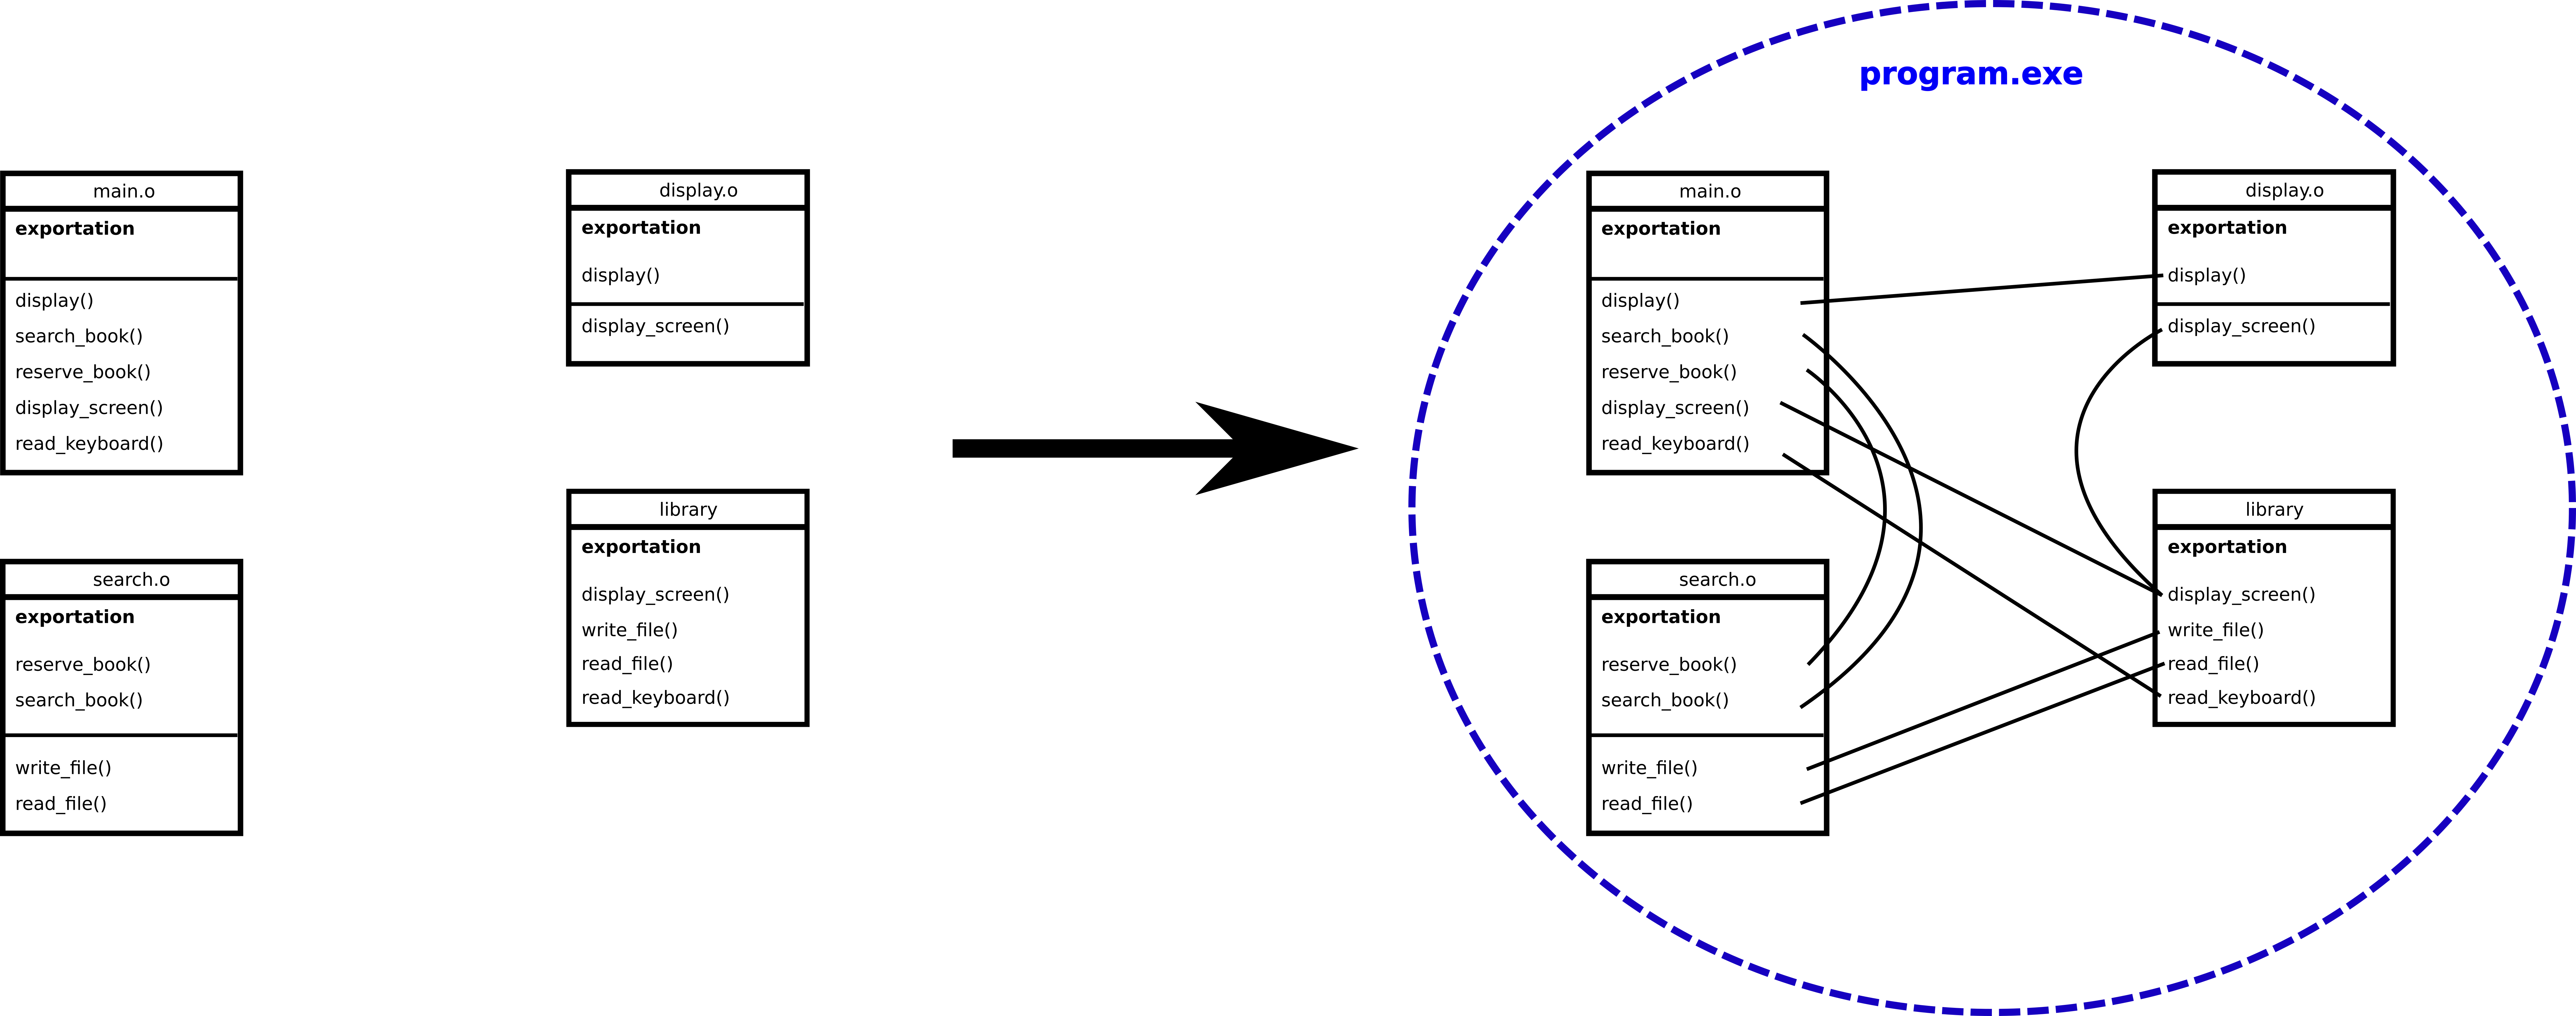
\includegraphics[scale=0.08]{images/link_editing.png} 
	\end{figure}
		
	\end{center}	
	
	\footnotetext[5]{The linker also link objects with external libraries (for instance, libraries to display windows)}
	
	\end{frame}
	
	\begin{frame}	
	
	Concretely the link editing process is as follows:
	\vspace*{1em}
	\begin{enumerate}
	\item{building a map of implementation}
	\item{building a table of links}
	\item{handling external libraries}
	\item{building the final executable}
	\end{enumerate}

	\end{frame}

	\begin{frame}
	
	\begin{block}{What is a map of implementation?}	
	It gives the \textbf{new starting addresses of each object}\footnotemark[5]	
	\end{block}
	
	Example of a building of a map of implementation:
	\vspace*{1em}	
	\begin{center}
	\begin{figure}
		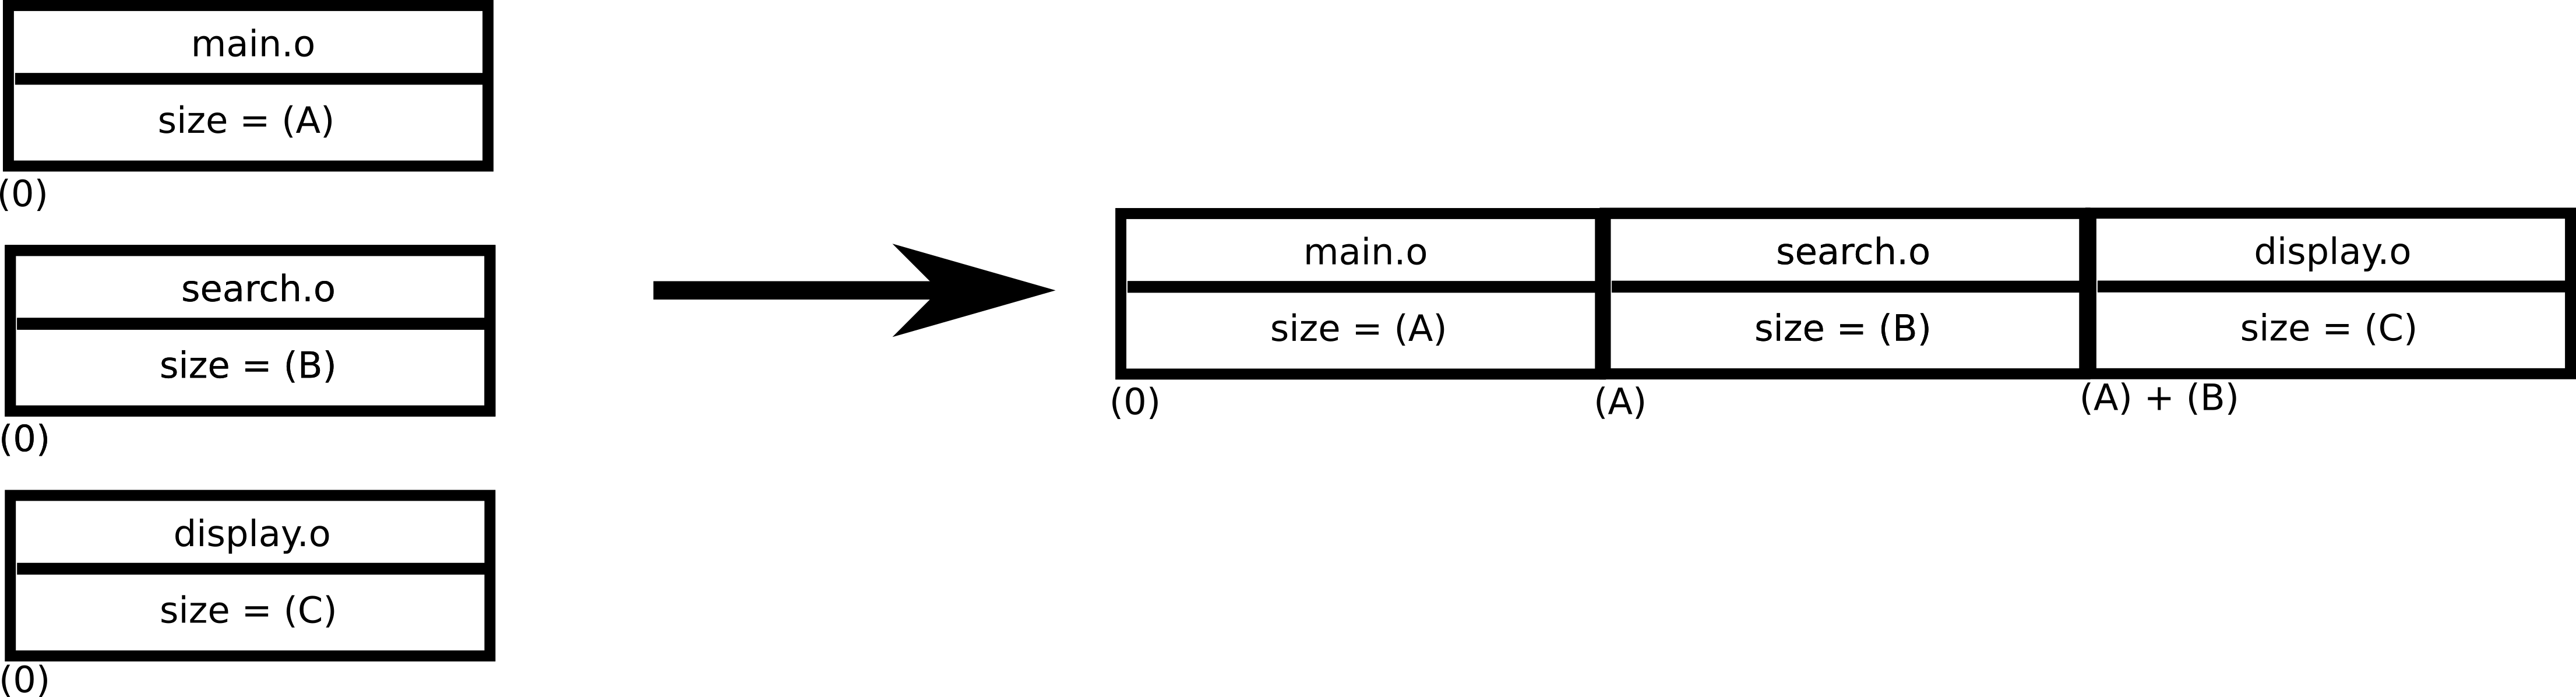
\includegraphics[scale=0.15]{images/map_of_implementation.png} 
	\end{figure}
	\end{center}

	\footnotetext[5]{Indeed, originally each module has (0) as a starting address}
	\end{frame}

	\begin{frame}

	\begin{block}{What is a table of links?}
	It \textbf{links the components} of the objects using the \textit{map of implementation}
	\end{block}	
	
	Example:	
	\vspace*{1em}
	
	\begin{columns}	
		
	\column{.5\textwidth}
	Before links are made:
	\vspace*{1em}	
	
	\scalebox{0.5} {
	\begin{tabular}{|c|c|}
	\hline
	\textbf{Name of component} & \textbf{Addresses} \\ \hline
	search\_book & UNDEFINED \\ \hline
	display & UNDEFINED \\ \hline
	reserve\_book & UNDEFINED \\ \hline
	read\_keyboard & UNDEFINED \\ \hline
	display\_screen & UNDEFINED \\ \hline
	read\_file & UNDEFINED \\ \hline
	write\_file & UNDEFINED \\ \hline
	\end{tabular}
	}
		
	\column{.5\textwidth}
	After links are made:
	\vspace*{1em}		
	
	\scalebox{0.5} {
	\begin{tabular}{|c|c|}
	\hline
	\textbf{Name of component} & \textbf{Addresses} \\ \hline
	search\_book & (A) + address\_search\_book \\ \hline
	display & (A) + (B) + address\_display \\ \hline
	reserve\_book & (A) + address\_reserve\_book \\ \hline
	read\_keyboard & UNDEFINED \\ \hline
	display\_screen & UNDEFINED \\ \hline
	read\_file & UNDEFINED \\ \hline
	write\_file & UNDEFINED \\ \hline
	\end{tabular}
	}
	\end{columns}
	
	\pause
	
	\vspace*{1em}	
	
	\begin{alertblock}{Some links are not yet resolved!}
	External libraries are not yet linked!
	\end{alertblock}
		
	\end{frame}

	\begin{frame}
	
	\textit{External libraries} can be linked in two ways:
	\vspace*{1em}
	\begin{itemize}
	\item{\textbf{statically}}
	\item{or later \textbf{when loaded in \textit{main memory}}}	
	\end{itemize}		
		
	\vspace*{1em}
	When \textit{external libraries} are statically linked:
	\vspace*{1em}	
	\begin{itemize}
	\item{\textbf{external libraries are added} to the final executable\footnotemark[6]}
	\item{the table of links is then updated as below\footnotemark[7]}
	\end{itemize}	 		
	
	\begin{center}
	\scalebox{0.5} {
	\begin{tabular}{|c|c|}
	\hline
	\textbf{Name of component} & \textbf{Addresses} \\ \hline
	search\_book & (A) + address\_search\_book \\ \hline
	display & (A) + (B) + address\_display \\ \hline
	reserve\_book & (A) + address\_reserve\_book \\ \hline
	read\_keyboard & (A) + (B) + (C) \\ \hline
	display\_screen & (A) + (B) + (C) + (D) \\ \hline
	read\_file & (A) + (B) + (C) + (D) + (E) \\ \hline
	write\_file & (A) + (B) + (C) + (D) + (E) + (F) \\ \hline
	\end{tabular}
	}	
	\end{center}
		
	\footnotetext[6]{The final executable becomes much bigger in size when statically linked}
	\footnotetext[7]{(D) = size \textit{read\_keyboard} library, (E) = size \textit{display\_screen} library, (F) = size \textit{read\_file} library}	
		
	\end{frame}
	
	\subsection{Loader}	
	
	\begin{frame}
	
	\begin{block}{What does the loader?}
	The loader...
	\begin{itemize}
	\item{...\textbf{changes the first address} of the executable}
	\item{...recalculate \textbf{internal component addresses}}
	\item{...load the \textbf{executable in \textit{main memory}}}
	\end{itemize}
	\end{block}
	
	\vspace*{1em}	
	
	\begin{columns}
	\column{.5\textwidth}
	New addresses:
	\begin{center}
	\scalebox{0.4} {
	\begin{tabular}{|c|c|}
	\hline
	\textbf{Name of component} & \textbf{Addresses} \\ \hline
				  & (offset) \\ \hline
	search\_book & (offset) + (A) + address\_search\_book \\ \hline
	display & (offset) + (A) + (B) + address\_display \\ \hline
	reserve\_book & (offset) + (A) + address\_reserve\_book \\ \hline
	read\_keyboard & (offset) + (A) + (B) + (C) \\ \hline
	display\_screen & (offset) + (A) + (B) + (C) + (D) \\ \hline
	read\_file & (offset) + (A) + (B) + (C) + (D) + (E) \\ \hline
	write\_file & (offset) + (A) + (B) + (C) + (D) + (E) + (F) \\ \hline
	\end{tabular}
	}	
	\end{center}
	
	\column{.5\textwidth}
	Loading the new executable:
	\begin{center}
	\begin{figure}
		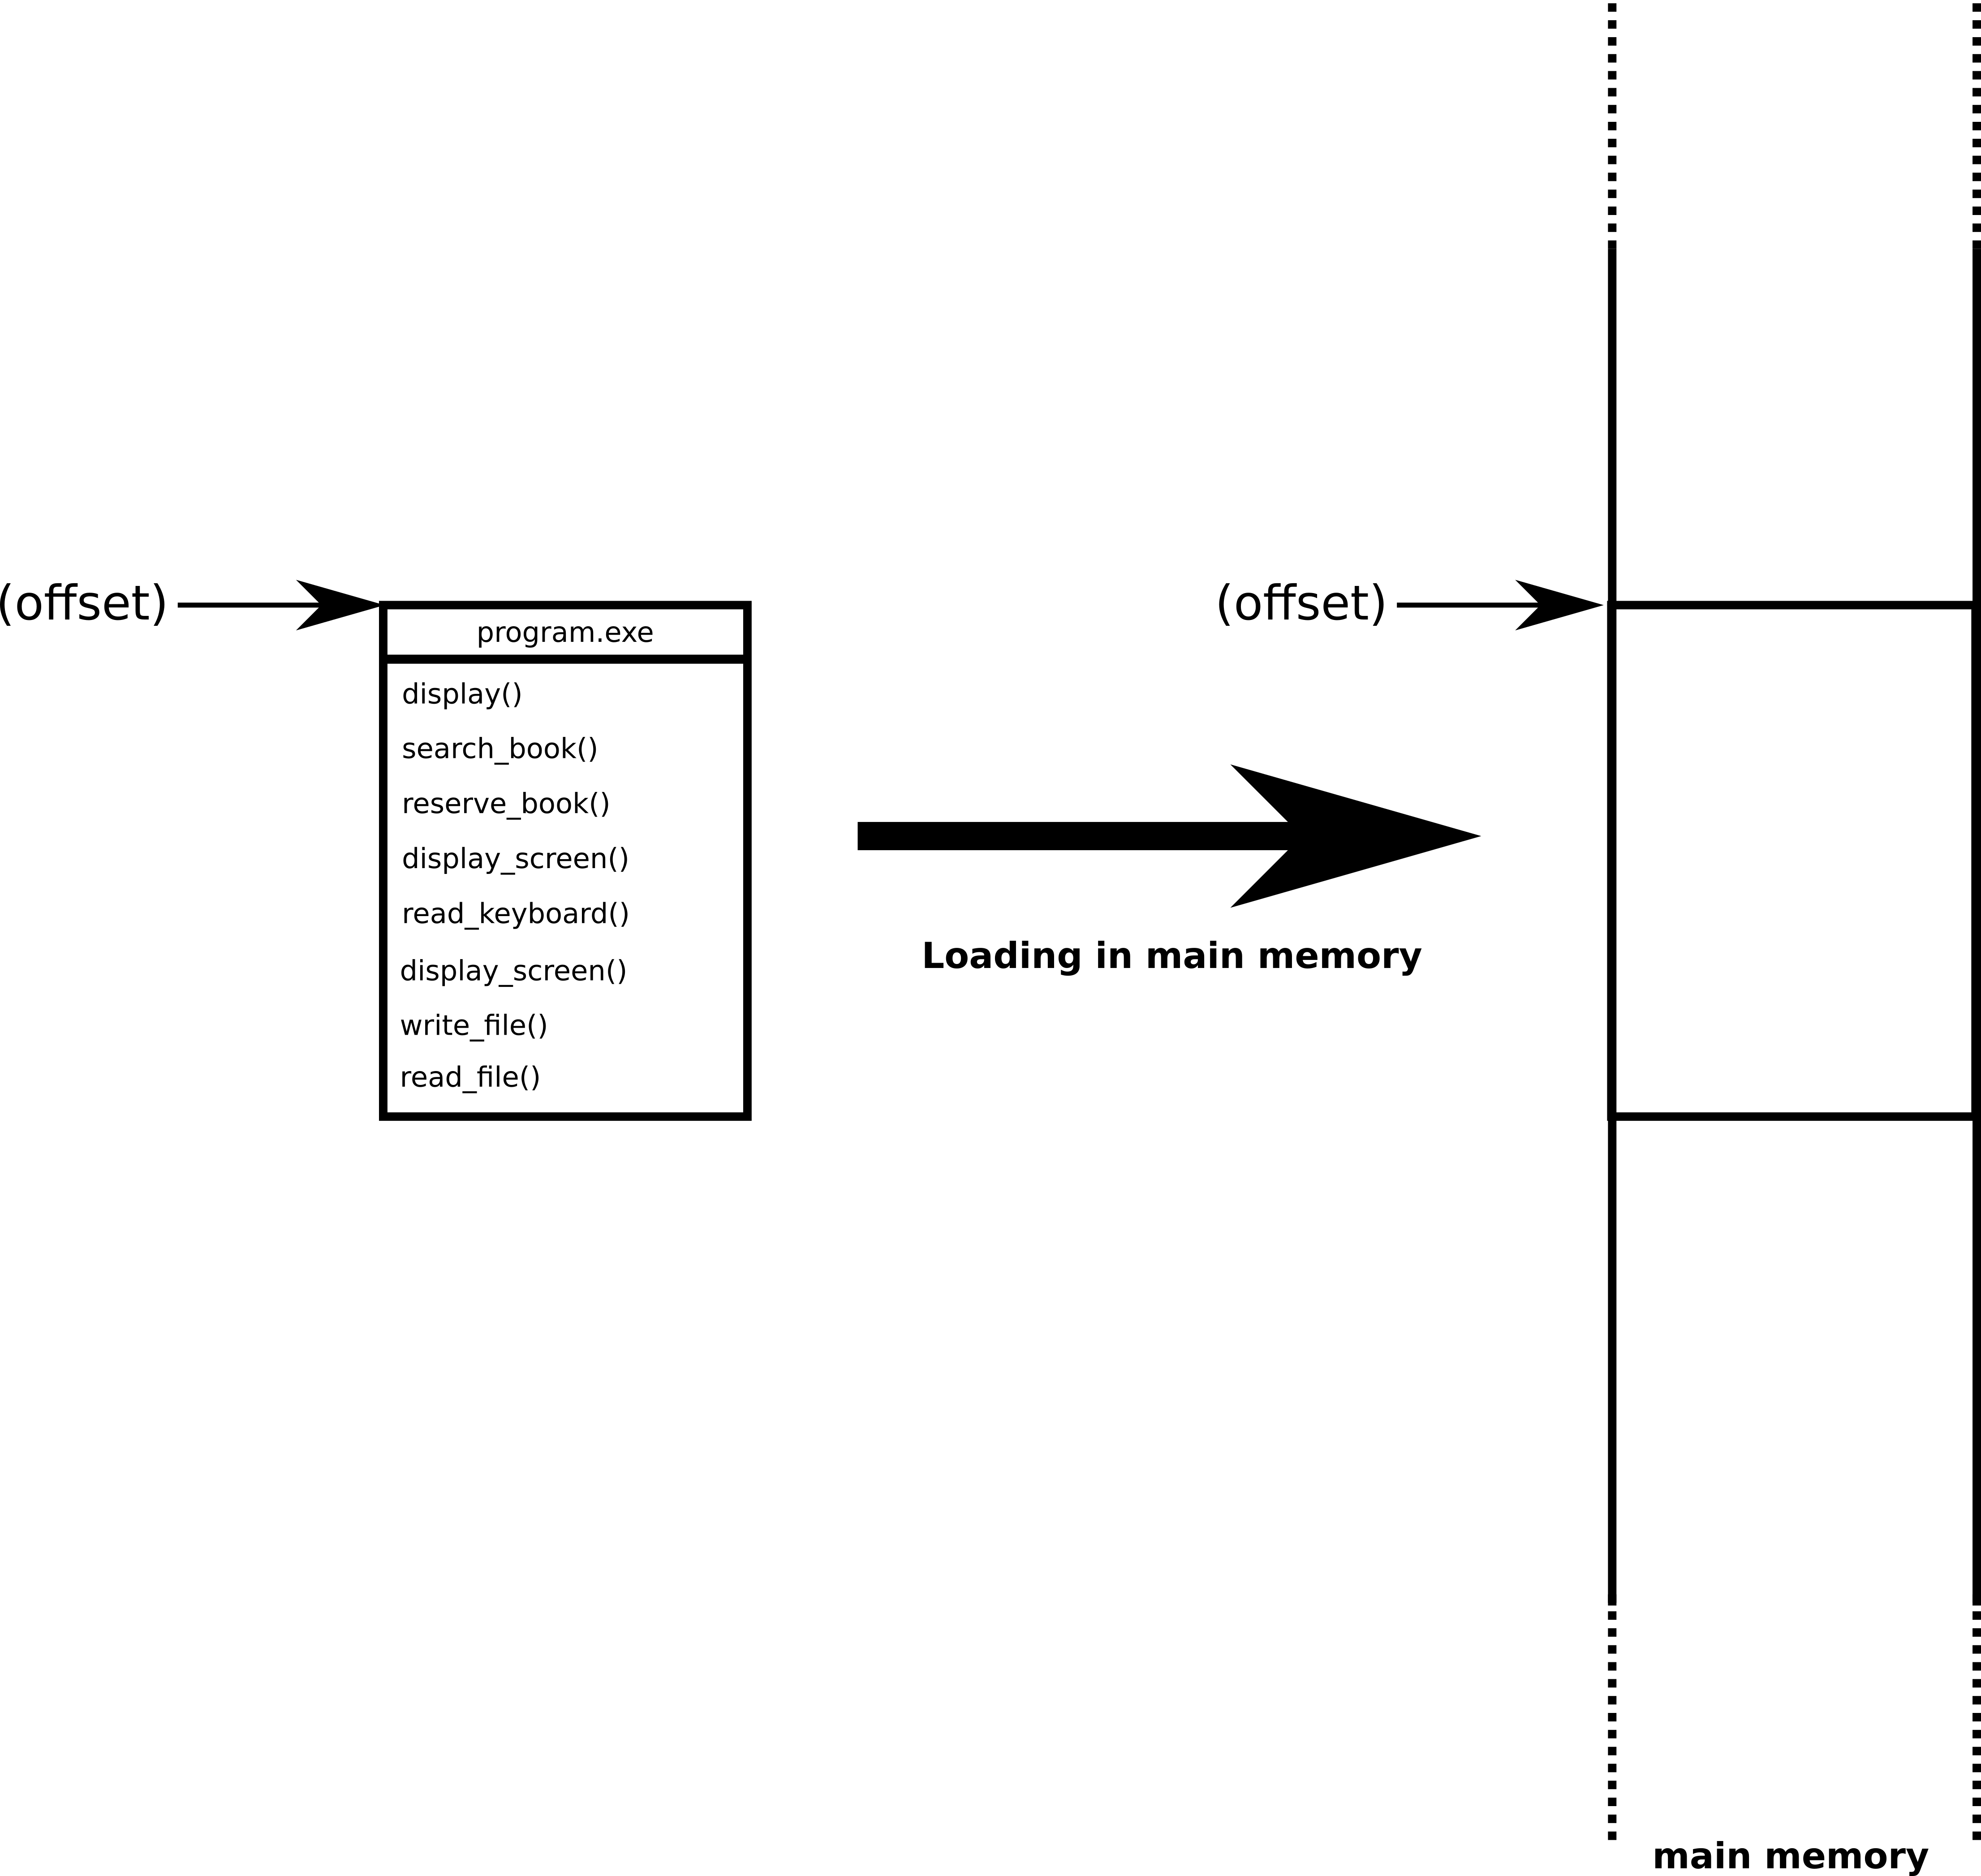
\includegraphics[scale=0.04]{images/loader.png} 
	\end{figure}
	\end{center}
	
	\end{columns}		
	
	\vspace*{1em}
	
	Now, the executable can be executed by the \textit{processor unit}\footnotemark[7]!
	
	\footnotetext[7]{The first address of the executable in \textit{main memory} is read by the processor unit}	
	
	\end{frame}

	\begin{frame}
	
	If libraries are dynamically linked, the loader will first:
	\vspace*{1em}
	\begin{enumerate}
	\item{\textbf{load independently the libraries} in \textit{main memory}}
	\item{\textbf{change the addresses in the table of links} accordingly}
	\end{enumerate}		
	
	\vspace*{1em}
	Example:
	\vspace*{1em}
		\begin{center}
	\scalebox{0.6} {
	\begin{tabular}{|c|c|}
	\hline
	\textbf{Name of component} & \textbf{Addresses} \\ \hline
				  & (offset) \\ \hline
	search\_book & (offset) + (A) + address\_search\_book \\ \hline
	display & (offset) + (A) + (B) + address\_display \\ \hline
	reserve\_book & (offset) + (A) + address\_reserve\_book \\ \hline
	read\_keyboard & (offset read\_keyboard) \\ \hline
	display\_screen & (offset display\_screen) \\ \hline
	read\_file & (offset read\_file) \\ \hline
	write\_file & (offset write\_file) \\ \hline
	\end{tabular}
	}	
	\end{center}
	\end{frame}


\end{document}
